\documentclass[11pt]{book}

\usepackage{fullpage}
\usepackage{graphicx}
\usepackage{cite}
\usepackage{times}
\usepackage{url}
\usepackage{setspace}
\usepackage{fancyhdr}
\usepackage{ifthen}
\usepackage{listings}
\usepackage[section]{placeins}
\usepackage{xtab}
\usepackage{url}
\usepackage{booktabs}
\usepackage{mathtools}
\usepackage{float}
\usepackage{morefloats}

\setcounter{topnumber}{2}
\setcounter{bottomnumber}{3}
\setcounter{totalnumber}{4}  
\renewcommand{\topfraction}{0.5}
\renewcommand{\bottomfraction}{0.95}
\renewcommand{\textfraction}{0.1}
\renewcommand{\floatpagefraction}{0.7}

\setlength{\abovecaptionskip}{3pt}
\setlength{\belowcaptionskip}{3pt}

\pagestyle{fancy}
\setboolean{@twoside}{false} 
\setlength{\headsep}{25pt}
\setlength{\headheight}{14pt}

\begin{document}

\thispagestyle{empty}

\doublespacing

\vspace*{0.5in}

\begin{center}
\LARGE{\textbf{Experiments with Hardware-based Transactional Memory in Parallel Simulation}}

\vspace*{0.4in}

  {\large A thesis submitted to the\\[0.20in]
    Division of Research and Advanced Studies\\
    of the University of Cincinnati\\[0.20in]
    in partial fulfillment of the\\
    requirements for the degree of\\[0.20in]
    {\bf MASTER OF SCIENCE}\\[0.20in]
    in the School of Electric and Computing Systems\\
    of the College of Engineering and Applied Sciences\\[0.20in]
    August xx, 2010\\[0.20in]
    by\\[0.20in]
    {\bf Joshua Hay}\\
    BSxx, University of Cincinnati, 20xx\\}
  \vspace{0.5in}
  {\large Thesis Advisor and Committee Chair:  Dr. Philip A. Wilsey}
\end{center}

\clearpage

\setcounter{page}{1}
\pagenumbering{roman}
\clearpage

\chapter*{Abstract} 

Transactional memory is a concurrency control mechanism that dynamically determines when
threads may safely execute critical sections of code.  It does so by tracking memory
accesses performed within a transactional region, or critical section, and detecting when
memory operations conflict with other threads.  Transactional memory provides the
performance of fine-grained locking mechanisms with the simplicity of coarse-grained
locking mechanisms.

Parallel Discrete Event Simulation is a problem space that has been studied for many
years, but still suffers from significant lock contention on SMP platforms.  The pending
event set is a crucial element to PDES, and its management is critical to simulation
performance.  This is especially true for optimistically synchronized PDES, such as those
implementing the Time Warp protocol.  Rather than prevent causality errors, events are
aggressively scheduled and executed until a causality error is detected.

This thesis explores the use of transactional memory as an alternative to conventional
synchronization mechanisms for managing the pending event set in a time warp synchronized
parallel simulator.  In particular, this thesis examines the use of Intel's hardware
transactional memory, TSX, to manage shared access to the pending event set by the
simulation threads.  In conjunction with transactional memory, other solutions to
contention are explored such as the use of multiple queues to hold the pending event set
and the binding of threads to these multiple queues.  The latter is an attempt to
decentralize the data structure holding pending event queue and distribute worker threads
among the decentralized data structure.  For each configuration a comparison between
conventional locking mechanisms and transactional memory access is performed to evaluate
each within the \textsc{warped} parallel simulation kernel.  In this testing, evaluation
of both forms of transactional memory (HLE and RTM) implemented in the Haswell
architecture were performed.  The results show that RTM generally performs on par with
conventional mutex locking primitives and that HLE provides consistently better
performance than conventional locking mechanisms.  HLE frequently outperforms conventional
locks by as much as 20\%.

\chapter*{Acknowledgments} 

%% put your acknowledgements here.


%% these three lines will cause latex to automatically generate these entries
%% for you....nice.  you can comment them out if, for example, your thesis does
%% not contain any tables.
\tableofcontents \markright{ }
\listoffigures \markright{ }
\listoftables \markright{ }

\clearpage
\pagenumbering{arabic} \setcounter{page}{1}

\chapter{Introduction}\label{intro} 

The advent of multi-core processors introduced a new avenue for increased software
performance and scalability through multi-threaded programming.  However, this avenue came
with a toll: the need for synchronization mechanisms between multiple threads of
execution, especially during the execution of critical sections.  By definition, a
critical section is a segment of code accessing a shared resource that can only be
executed by one thread at any given time \cite{os_concepts}.  For example, consider a
multi-threaded application that is designed to operate on a shared two-dimensional array.
For the sake of simplicity, the programmer uses coarse-grained locking mechanisms to
control access to the critical section, \emph{e.g.,} a single atomic lock for the entire
structure.  The critical section reads a single element, performs a calculation, and
updates the element of the array.  Once a thread enters the critical section, it locks all
other threads out of the entire array until it has completed its task, thus forcing the
collection of threads to essentially execute sequentially through the critical section
even when they are accessing completely independent subparts of the array.  This results
in lock contention, and consequently negatively impacts performance, as threads must now
wait for the currently executing thread to relinquish access to the shared resource.
Programmers can employ more fine-grained locking mechanisms to expose concurrency, such as
locking individual rows or even individual elements in the previous example.  However,
this approach is vastly more complicated and error prone \cite{sle_rajwar}; this approach
requires the programmer to define and maintain a separate lock for each row or each
element.  Unfortunately, programmers are limited to using static information to decide
when threads must execute a critical section regardless of whether coarse-grained or
fine-grained locking is used.

In the previous example, a scenario arises where one thread will access one element of the
two dimensional array, while another thread will access a element in an entirely different
row.  The programmer only knows that any thread can access any given element at any given
time, and thus locks all elements when one thread is executing the critical
section. Untapped concurrency can be exposed if the decision to execute a critical section
made dynamically \cite{intel_prog_ref}.

%% This paragraph is still highly confusing.  we can leave it for now, but it remains a
%% poor introduction of transactional memory.  if the reader really needs this
%% information, your prose would not make it clear to them....  the paragraph below this
%% is actually a better introduction.

Transactional memory (TM) is a concurrency control mechanism that attempts to eliminate
the static sequential execution of a critical section by dynamically determining when
accesses to shared resources can be executed concurrently \cite{sle_rajwar}.  In the
previous example, instead of using locks, the programmer identifies the critical section
as a transactional region (hereafter, the terms, \emph{critical region} and
\emph{transaction} will be used interchangeably).  As the threads enter the transactional
region, they attempt to ``atomically'' execute the critical section.  The TM system
records memory accesses as the transactions execute and finds that the transactions
operate on independent regions of the data structure, \emph{i.e.,} there are no
conflicting memory accesses.  Instead of being forced to execute sequentially by the
programmer, the threads are allowed to concurrently and safely execute the critical
section.  Transactional memory is analogous to traffic roundabouts whereas conventional
synchronization mechanisms are analogous to conventional traffic lights
\cite{neuling_vid}.

Transactional memory operates on the same principles as database transactions
\cite{tm_2nd}.  The processor atomically commits \emph{all} memory operations of a
successful transaction or discards \emph{all} memory operations if the transaction should
fail (a collision to the updates by the multiple threads occurs).  In order for a
transaction to execute successfully, it must be executed in isolation, \emph{i.e.,}
without conflicting with other tranasctions/threads memory operations.  This is the key
principle that allows transactional memory to expose untapped concurrency in
multi-threaded applications.

One problem space that could benefit from transactional memory is that of Parallel
Discrete Event Simulation (PDES).  In Discrete Event Simulation (DES) applications, a
physical system is modeled as a collection of Logical Processes (LPs) representing the
physical processes of the system.  The system being modeled can only change state at
discrete points in simulated time and only changes state upon execution of an event
\cite{fujimoto}.  Large simulations, such as those in economics, engineering, and military
tactics, require enormous resources and computational time, making it infeasible to
execute them on sequential machines.  The necessity to perform such large simulations has
sparked considerable interest in the parallelization of these simulations.  In PDES, the
events of the LPs are executed concurrently.  To further exploit concurrency, optimistic
PDES aggressively schedules events instead of strictly enforcing causal ordering of event
execution \cite{fujimoto,dickman_thesis}.  This means that events will continue to be
scheduled without strict enforcement of their causal order until a causal violation is
\emph{detected}.  More importantly, the events must be retrieved from a global (and
shared) pending event set by one of multiple execution threads, resulting in non-trivial
contention for this structure.  A key challenge area in PDES is the need for
contention-free pending event set management solutions \cite{dickman}; this will be the
primary focus of this research.  Transactional memory can help alleviate contention for
this shared structure and expose untapped concurrency in the simulation's execution.

Researchers at the University of Cincinnati have developed a PDES kernel called
\textsc{warped}, that implements the optimistic Time Warp synchronization protocol
\cite{jefferson-85,fujimoto}.  In \textsc{warped}, events to be scheduled are sorted into
a global Least-Time-Stamp-First (LTSF) queue.  When a worker thread schedules an event, it
locks the LTSF queue and retrieves the event from the head of the queue.  Thus, the LTSF
becomes the primary source of contention in the \textsc{warped} kernel.

\section{Research Statement}

The goal of this thesis is to explore the use of transactional memory in a parallel
discrete event simulator.  In particular, experiments with transactional memory to manage
access to the pending event set data structures of the \textsc{warped} parallel discrete
event simulation enging are examined.

The primary objective of this research is to \emph{modify the \textsc{warped} pending
  event set locking mechanisms to utilize the underlying hardware support for
  transactional memory on Intel's Hardware Transactional Memory (HTM) supported Haswell
  platform}.  The principal hypothesis is that making the aforementioned modifications
will exposed untapped concurrency during simulation execution, thereby improving the
performance of \textsc{warped} on the Haswell platform.

Due to the wide availability of Intel's HTM supported platforms, it was selected as the
focus of this research.  Intel's HTM implementation is aptly named Transactional
Synchronization Extensions (TSX).  This naming will be used to refer to Intel's HTM
implementation for the remainder of this study.

While \textsc{warped} uses many shared data structures, the focus of this thesis is on the
pending event set.  It is the primary bottleneck in PDES applications, and hence the
primary motivation for this study.

\section{Thesis Overview}

The remainder of this thesis is organized as follows:

Chapter 2 provides a general overview of transactional memory.  It gives some examples of
other TM implementations and discusses why they do not work as well as TSX.  It provides
examples of related studies.  Finally, it provides an overview of how TSX works and how it
is implemented in software.

Chapter 3 discusses practical considerations for the programmer when programming TSX
enabled multi-threaded applications.  It discusses optimizations to ensure TSX performs
optimally, as well as physical limitations of the hardware.

Chapter 4 provides a background of the PDES problem space.  It introduces \textsc{warped}
and some of the implementation details relevant to this study.  Previous studies with the
\textsc{warped} pending event set are also briefly discussed.

Chapter 5 discusses how TSX is implemented in \textsc{warped}.  It also provides a brief
overview of the critical sections utilizing TSX and why TSX will be beneficial.

Chapter 6 provides and discusses the experimental results of this research for several
different simulation configurations.

Chapter 7 discusses the accomplishments of this research.  It also briefly discusses some
areas of future research.


\chapter{Background}

yaoi1023
This section provides a high level explanation of how transactional memory operates.  It
then introduces other implementations, as well as reasons why they were not explored in
this study.  Next, it provides some examples of related studies with transactional memory,
specifically the implementation used in this study.  Finally, it provides an overview of
Intel's implementation, Transactional Synchronization Extensions (TSX) and how the
programmer can develop TSX enabled multi-threaded applications.

\section{Transactional Memory Overview}

Transactional memory (TM) is a concurrency control mechanism that dynamically determines
when two or more threads can safely execute a critical section \cite{sle_rajwar}.  The
programmer identifies a transactional region, typically a critical section, for
monitoring.  When the transaction executes, the TM system, whether it is implemented in
hardware or software, tracks memory operations performed within the transactional region
to determine whether or not two or more transactions conflict with one another,
\emph{i.e.,} if any memory accesses conflict with one another.  If the threads do not
conflict with one another, the transactions can be safely and concurrently executed.  If
they do conflict, the process must abort the transaction and execute the critical section
non-transactionally, \emph{i.e.,} by serializing execution of the critical section with
conventional synchronization mechanisms.

%% JOSH: review this rewritten paragraph and verify/correct it accordingly.
%%As a transaction is executed, the processor buffers the memory write operations and
%%commits them only when the transaction is complete and safe access has been determined.
%%Safe access is determined by the processor core by recording the set memory read addresses
%%(called the \emph{read-set}) and memory write addresses (called the \emph{write-set}) from
%%the instructions in the transaction.  During the time of the transaction memory addresses
%%of instructions executed by other concurrently executed threads are also recorded.  If
%%there is an intersection of the addresses from the transaction with addresses from any of
%%the concurrently executed threads, the transaction aborts (safe access did \emph{not}
%%occur).  Upon completing a transaction with safe access, the transaction will atomically
%%commit all of the buffered memory operations, henceforth referred to simply as a
%%\emph{commit}.

%% JOSH: here's a question, what happens if the code accesses a shared memory region
%% outside of a transaction (say it reads it); does this get considered in the validity of
%% the transaction?  or would it simply commit?

%% Dr. Wilsey: It is my understanding that ANY memory operation performed
%% during transactional execution is tracked by the TM system.  So if a shared
%% memory region is accessed outside of a transaction (which I'm not 100% sure what
%% you mean by that). it will still be added to the transactions read-set for
%% conflict detection.

%% JOSH: outside of a transaction means exactly that, a memory reference that is not
%% contained within a transction (critical region).  
%%
%% ok, now that we have established that the tracking of memory references outside of a
%% transaction do indeed happen, i have two comments:
%% (1) you should revise the prose below to make that fact more clear in your description
%%     of (at least the haswell implementation of) transactional memory.
%% (2) would there be any performance benefit of skipping the use of the transaction
%%     operations for a read to a shared variable?  if so, what can/should we say about
%%     that?

As a transaction is executed, the memory operations performed within the transaction are
buffered, specifically write operations.  Write operations will only be fully committed
when the transaction is complete and safe access has been determined.  Safe access is
determined by comparing the set of addresses each transaction reads from (called the
\emph{read-set} and the set of addresses each transation writes to (called the
\emph{write-set}).  Each transaction builds its own read-set and write-set as it executes.
The TM system compares the read-sets and write-sets of all concurrently executing
transactions to determine if any memory operations conflict.  If the transaction completes
execution and the TM system has not detected any conflicting memory operations, the
transaction atomically commits all of hte buffered memory operations, henceforth referred
to simply as a \emph{commit}.

Whenever safe access does not occur, the transaction cannot safely continue execution.
This is referred to as a \emph{data conflict} and only occurs if: (i) one transaction
attempts to read a location that is part of another transaction's write-set, or (ii) a
transaction attempts to write a location that is part of another transaction's read-set
\cite{intel_prog_ref}.  Once a memory location is written to by a transaction, it cannot
be accessed in any way by any other transaction; any access by any other transaction
results in a race condition.  If such a situation arises, all concurrently executing
transactions will abort execution, henceforth referred to simply as an \emph{abort}.

Revisiting the example from Chapter \ref{intro}, assume that a programmer uses
transactional memory synchronization mechanisms to access a shared two dimensional array.
Recall that any thread can access any element at any given time.  One thread enters the
transactional region and begins transactional execution.  It adds the element's memory
location to its read-set.  At the same time, another thread enters the transactional
region; however, it accesses a different element.  As the first thread continues
execution, it adds the element's memory location to its write-set.  The second thread adds
its element's memory location to its read-set at the same time.  However, because the
memory location is not part of the first thread's read-set, the threads continue executing
concurrently.  No memory conflicts are detected in this case and the transactions execute
successfully and commit.

Now, assume that another thread enters the transactional region.  It begins its read
operation on a specific element and adds the element memory address to the read-set.
However, another thread is is already writing to that memory location.  Because the memory
address is tracked in the second transaction's write-set, a data conflict occurs.  The two
threads cannot execute concurrently and be guaranteed to produce the correct output.
Therefore, the transactions must abort.  Typically, the threads will retry execution with
explicit synchronization.  Although, as will be shown later, various retry options are
possible. 

By definition, a transaction is a series of actions that appears instantaneous and
indivisible possessing four key attributes: (1) atomicity, (2) consistency, (3) isolation,
and (4) durability \cite{tm_2nd}.  TM operates on the principles of database transactions.
The two key attributes for TM are atomicity and isolation; consistency and durability must
hold for all multi-threaded operations in multi-threaded applications.  Atomicity is
guaranteed if: (1) all memory operations performed within the transaction are completed
successfully, or (2) it appears as if the performed memory operations were never attempted
\cite{tm_2nd}.  Isolation is guaranteed by tracking memory operations as the transactions
execute and aborting if any memory operations conflict.  If both atomicity and isolation
can be guaranteed for all memory operations performed within a critical section, that
``critical section'' can be executed concurrently \cite{sle_rajwar}.

In the case of a commit, the transaction has ensured that its memory operations are
executed in isolation from other threads and that \emph{all} of its memory operations are
committed, thus satisfying the isolation and atomicity principles.  Note that only at this
time will the memory operations performed within the transaction become visible to other
threads, thus satisfying the appearance of instantaneousness.  In the case of an abort due
to a data conflict, it is clear that the isolation principle has been violated.  It should
be noted that transactions can abort for a variety of reasons depending on the
implementation \cite{intel_opt_man,chung_amd}, but the primary cause is data conflicts.
Upon abort, all memory operations are discarded to maintain atomicity.

\section{Related Studies}

There have been many implementations of TM systems since its conception mostly in software
\cite{yoo_tsx,chitters_tsx,rock_dice,chung_amd,blue_wang,quake_stm,stm_cascaval}.  As the
name suggests, Software Transactional Memory (STM) systems implement the memory tracking,
conflict detection, write buffering and so on in software.  Most systems are
implementation specific, but memory tracking is typically done through some form of
logging.  While this allows transactional memory enabled applications to be executed on a
variety of platforms, performance usually suffers.  Gajinov \emph{et al} performed a study
with STM by developing a parallel version of the Quake multi-player game server from the
ground up using OpenMP parallelizations pragmas and atomic blocks \cite{quake_stm}.  Their
results showed that the logging overhead required for STM resulted in execution times that
were 4 to 6 times longer than the sequential version of the server.  In general, STM has
been found to result in significant slowdown \cite{stm_cascaval}.  Although STM is more
widely available than HTM, its use in this this study was dismissed due to the significant
performance penalty.

Hardware Transactional Memory (HTM) provides the physical resources necessary to implement
transactional memory effectively.  Many chip manufacturers have added, or at least sought
to add, support for HTM in recent years.  IBM released one of the first commercially
available HTM systems in their Blue Gene/Q machine \cite{blue_wang}.  Even though they
found that this implementation was an improvement over STM, it still incurred significant
overhead.  AMD's Advanced Synchronization Facility and Sun's Rock processor included
support for HTM \cite{chung_amd,rock_dice}.  However, AMD has not released any HTM enabled
processors and Sun's Rock processor was canceled after Sun was acquired by Oracle.

With the release of Intel's Haswell generation processors, Intel's Transactional
Synchronization Extensions (TSX) is the currently the only widely available commercial
HTM-enabled system.  Numerous studies have already been performed with TSX, primarily
evaluating its performance capabilities.  Chitters \emph{et al} modified Google's write
optimized persistent key-value store, LevelDB, to use TSX based synchronization instead of
a global mutex.  Their implementation shower 20-25\% increased throughput for write-only
workloads and increased throughput for 50\% read / 50\% write workloads
\cite{chitters_tsx}.  Wang \emph{et al} studied the performance scalability of a
concurrent skip-list using TSX Restricted Transactional Memory (RTM).  They compared the
TSX implementation to a fine-grain locking implementation and a lock-free implementation.
They found that the performance was comparable to the lock-free implementation without the
added complexity \cite{wang_tsx}.  Yoo \emph{et al} evaluated the performance of TSX using
high-performance computing (HPC) workloads, as well as in a user-level TCP/IP stack.  They
measured an average speed up of 1.41x and 1.31x respectively \cite{yoo_tsx}.  The decision
to use Intel's TSX for this research was based on its wide availability and the
performance improvements observed in other studies.

\section{Transactional Synchronization Extensions (TSX)}

Intel's Transactional Synchronization Extensions (TSX) is an extension to the x86
instruction set architecture that adds support for HTM.  TSX operates in the L1 cache
using the cache coherence protocol \cite{intel_opt_man}.  It is a best effort
implementation, meaning it does not guarantee transactions will commit
\cite{intel_prog_ref}.  TSX has two interfaces: (1) Hardware Lock Elision (HLE), and (2)
Restricted Transactional Memory (RTM).  While both operate on the same principles of
transactional memory, they have subtle differences.  This section discusses some of the
implementation details of TSX as well as how the programmer utilizes TSX.

\subsection{Hardware Lock Elision (HLE)}\label{sec:hle}

The Hardware Lock Elision (HLE) interface is a legacy-compatible interface introducing two
instruction prefixes, namely: 

\vspace*{-\bigskipamount}
\begin{singlespace}
\begin{enumerate}
  \item \texttt{XACQUIRE} and 
  \item \texttt{XRELEASE}.
\end{enumerate}
\end{singlespace}

\noindent
The \texttt{XACQUIRE} prefix is placed before a locking instruction to mark the beginning
of a transaction.  \texttt{XRELEASE} is placed before an unlocking instruction to mark the
end of a transaction.

These prefixes tell the processor to elide the write operation to the lock variable during
lock acquisition/release.  When the processor encounters an \texttt{XACQUIRE} prefixed
lock instruction, it transitions to transactional execution.  Specifically, it adds the
lock variable to the transaction's read-set instead of issuing any write requests to the
lock \cite{intel_prog_ref}.  To other threads, the lock will appear to be free, thus
allowing those threads to enter the critical section and execute concurrently.  All
transactions can execute concurrently as long as no transactions abort and explicitly
write to the lock variable.  If that were to happen, a data conflict technically occurs
--- one transaction writes to a memory location (the lock) that is part of another
transaction's read-set.

The \texttt{XRELEASE} prefix is placed before the instruction used to release the lock.
It also attempts to elide the write associated with the lock release instruction.  If the
lock release instruction attempts to restore the lock to the value it had prior to the
\texttt{XACQUIRE} prefixed locking instruction, the write operation on the lock is elided
\cite{intel_prog_ref}.  It is at this time that the processor attempts to commit the
transaction.

However, if the transaction aborts for any reason, the region will be re-executed
non-transactionally.  If the processor encounters an abort condition, it will discard all
memory operations performed within the transaction, return to the locking instruction, and
resume execution without lock elision, \emph{i.e.,} the write operation will be performed
on the lock variable.  If any other thread is executing the same transactional region,
those transactions will also abort.  The aborted transaction thread performs an explicit
write on the lock, resulting in a data conflict for any other transaction as the lock
variable is part of the other transaction's read-set.  The re-execution of the critical
section using conventional synchronization is necessary to guarantee forward progress
\cite{intel_prog_ref}.

An example of a standard locked critical section using the x86 atomic exchange instruction
is shown in Figure~\ref{fig:lock_interface} (as a reference for the TSX HLE interfaces
shown below).  The \texttt{\_\_atomic\_exchange\_n(type *ptr, type val, int memmodel}
intrinsic implements the atomic exchange operation as the name suggests.  It writes
\texttt{val} into \texttt{ptr} and returns the previous contents of \texttt{ptr}.  The
most important parameter is \texttt{memmodel}; it specifies synchronization requirements
between threads.  For instance, the \_\_ATOMIC\_ACQUIRE memory model synchronizes the
local thread with a release semantic store from another thread \cite{gcc}.  Essentially,
when another thread executes a lock release, the local thread will execute the lock
acquire.  The while loop further ensures the lock is free before it is acquired (the
while loop repeats the \texttt{\_\_atomic\_exchange\_n} operation until the lock is
aquired). 

\begin{figure}
\begin{verbatim}
/* Acquire lock */
/* Loop until the returned val indicates the lock was free */
while(__atomic_exchange_n(&lock, 1, __ATOMIC_ACQUIRE)):

/* Begin executing critical section */
...
/* End critical section */

/* Free lock */
__atomic_store_n(&lock, 0,__ATOMIC_RELEASE);
\end{verbatim}
    \caption{\textbf{Standard Atomic Lock Implementation}}\label{fig:lock_interface} 
\end{figure}

To enable HLE synchronization, the programmer merely adds the HLE memory models to the
existing locking intrinsics (Figure~\ref{fig:hle_interface}).  The
\_\_ATOMIC\_HLE\_ACQUIRE tells the thread to execute an \texttt{XACQUIRE} prefixed lock
acquire instruction when another thread releases the lock.  The combination of memory
models, \texttt{\_\_ATOMIC\_HLE\_ACQUIRE|\_\_ATOMIC\_HLE\_ACQUIRE)} allows for the locking
instructions to be executed with or without elision.  The local thread can be synchronized
to a \texttt{XRELEASE} prefixed lock release instruction or a standard lock release
instruction.

\begin{figure}
\begin{verbatim}
/* Acquire lock with lock elision if possible */
/* Loop until the returned val indicates the lock was free */
while(__atomic_exchange_n(&lock, 1, __ATOMIC_HLE_ACQUIRE|__ATOMIC_ACQUIRE)):

/* Begin executing critical section/transactional region */
...
/* End critical section/transactional region */

/* Free lock with lock elision if possible */
__atomic_store_n(&lock, 0, __ATOMIC_HLE_RELEASE|__ATOMIC_RELEASE);
\end{verbatim}
    \caption{\textbf{Generic HLE Software Implemenation}}\label{fig:hle_interface}
\end{figure}

HLE is legacy compatible.  Code utilizing the HLE interface can be executed on legacy
hardware, but the HLE prefixes will be ignored \cite{intel_prog_ref} and the processor
will always perform the write operation on the locking variable and execute the critical
section non-transactionally.  While this interface does nothing for multi-threaded
applications on legacy hardware, it does allow for easier cross-platform code deployment.

\subsection{Restricted Transactional Memory (RTM)}\label{sec:rtm}

The Restricted Transactional Memory (RTM) interface for HTM introduces four new
instructions, namely: 

\vspace*{-\bigskipamount}
\begin{singlespace}
\begin{enumerate}
  \item \texttt{XBEGIN}, 
  \item \texttt{XEND}, 
  \item \texttt{XABORT}, and 
  \item \texttt{XTEST}.
\end{enumerate}
\end{singlespace}

\noindent
The \texttt{XBEGIN} instruction marks the start of a transaction, while the \texttt{XEND}
instruction makes the end of a transaction.  The \texttt{XABORT} instruction is used by
the programmer to manually abort a transaction.  Finally, the \texttt{XTEST} instruction
can be used to test if the processor is executing transactionally or non-transactionally.

The \texttt{XBEGIN} instruction transitions the processor into transactional execution
\cite{intel_prog_ref}.  Note that the \texttt{XBEGIN} instruction does not elide the
locking variable as HLE does.  Therefore, the programmer should manually add the locking
variable to the transaction's read-set by checking if the lock is free at the start of the
transaction.  If it is free, the transaction can execute safely.  Once execution reaches
the \texttt{XEND} instruction, the processor will attempt to commit the transaction.

As previously mentioned, the transaction can abort for many reasons.  One case specific to
RTM occurs when the lock is not free upon entering the transaction.  In this case, the
programmer uses the \texttt{XABORT} instruction to explicitly abort the transaction.  But
no matter the reason for the abort, execution jumps to the fallback instruction address
\cite{intel_prog_ref}.  This address is specified as an operand of the \texttt{XBEGIN}
instruction.

It is this fallback path that makes RTM a much more flexible interface than HLE because it
is entirely at the discretion of the programmer to determine precisely what happens on
failure of a transaction.  Even so, the programmer must still provide an abort path that
guarantees forward progress \cite{intel_prog_ref}.  Therefore, the abort path should use
explicit synchronization, \emph{e.g.,} acquire the lock, to ensure forward progress.
However, the programmer can use this abort path to tune the performance of RTM enabled
applications.  For instance, a retry routine can be used to specify how many times the
processor should attempt to enter transactional execution before using explicit
synchronization.  Furthermore, the \texttt{EAX} register reports information about the
condition of an abort \cite{intel_prog_ref}, such as whether or not the abort was caused
by the \texttt{XABORT} instruction, a data conflict, and so on.  The programmer can use
this information to make more informed decisions regarding reattempting transactional
execution.

\begin{figure}
\begin{verbatim}
if (_xbegin() == _XBEGIN_STARTED) {
    /* Add lock to read-set */
    if (lock is not free) {
        /* Abort if lock is already acquired */
        _xabort(_ABORT_LOCK_BUSY);
    }
} else {
    /* Abort path */
    acquire lock
}

/* Begin critical section/transactional region */
...
/* End critical section/transactional region */

if (lock is free) {
    /* End transaction and commit results*/
    _xend();
} else {
    release lock
}
\end{verbatim}
    \caption{\textbf{Generic RTM Software Implementation}}\label{fig:rtm_interface}
\end{figure}

The RTM implementation is more involved because it uses entirely new instructions.  The
general algorithm for the RTM software interface is shown in
Figure~\ref{fig:rtm_interface}.  The programmer moves the existing locking mechanism
inside an else clause of the \texttt{XBEGIN} if statement, which will determine if the
processor transitions to transactional execution or takes the abort path.  As previously
mentioned, the processor will also return to this point should the transaction abort in
the middle of execution.  Moving the locking mechanism into the RTM abort path ensures
that the abort path ultimately uses explicit synchronization and guarantees forward
progress.  GCC 4.8 and above includes support for the \texttt{\_xbegin},
\texttt{\_xabort}, and \texttt{\_xend} intrinsics to implement the associated instructions
\cite{gcc}.

While RTM is a much more flexible interface than HLE, it can only be used on supported
Haswell platforms.  If a legacy device attempts to execute one of the RTM instructions, it
will throw a General Protection Fault.  It should be noted that execution of the
\texttt{XEND} instruction outside of a transaction will result in a General Protection
Fault as well \cite{intel_opt_man}.

\chapter{Practical Programming with TSX}

Before implementing TSX in the \textsc{warped} simulation kernel, a more in depth
evaluation of its capabilities needed to be performed.  One of the disadvantages of HTM is
the physical limitations of the hardware.  This section evaluates practical programming
techniques to consider when using TSX to ensure optimal performance.  Custom benchmarks
were developed to evaluate these various constraints.  All benchmarks were run on a system
with an Intel i7-4770 running at 3.4GHz with 32 GB RAM.  Each core has a 32KB 8-way, set
associative L1 cache and a 256 L2 cache.  Each cache line is 64 bytes.  This information
was verified using common Unix commands.  All measurements were performed ten times and
averaged.  This discussion of this chapter is directly related to the Intel Haswell
i7-4770 processor implementation of HTM.  Generalization of these results and the
corresponding discussion to other processor implementations of HTM should not be made. 

\section{Memory Organization}

TSX maintains a read-set and a write-set with the granularity of a cache line
\cite{intel_prog_ref}.  During transactional execution, TSX constructs a record of memory
addresses read from and a record of memory addresses written to.  A data conflict occurs
if another thread attempts to (i) read an address in the write-set or (ii) write an
address in the read-set.  This definition can be expanded to state that \emph{a data
  conflict} occurs if:

\vspace*{-\bigskipamount}
\begin{singlespace}
\begin{enumerate}
  \item another thread attempts to read a memory address that occupies the same cache line
    as a memory address to be written, or
  \item another thread attempts to write a memory address that occupies the same cache
    line as a memory address that has been read from.
\end{enumerate}
\end{singlespace}

\noindent
Therefore, aborts can be caused by data occupying the same cache line, essentially
reporting a false conflict on the shared data \cite{intel_opt_man}.  To mitigate the
effects of shared cache line data conflicts, the programmer must be conscientious of how
data is organized in memory.  For instance, the data in the previously discussed
benchmarks is optimally organized by allocating individual elements to 64 bytes,
\emph{i.e.,} a single cache line.

Furthermore, data elements should be aligned to cache line boundaries to ensure that each
element is limited to exactly one cache line.  If a data element crosses a cache line
boundary, the probability of shared cache line data conflicts increases as the data access
now has to check against two cache lines.

\section{Transaction Size}

TSX maintains a transaction read-set and write-set in the L1 cache \cite{intel_opt_man}.
The size of these memory sets is therefore limited by the size of the L1 cache.
Hyper-threading further restricts the size of the transaction data sets because the L1
cache is shared between two threads on the same core \cite{intel_opt_man}.  Based on
granularity of the read-set and write-set stated above, the transaction size is defined as
the number of cache lines accessed within a transaction.

The first two benchmarks evaluate the size restrictions of a transaction's read-set and
write-set, \emph{i.e.,} how many cache lines can a transaction track in each set during
transactional execution.  The benchmarks access a shared array of custom structures.  Each
structure is allocated to occupy an entire cache line and aligned to the nearest cache
line boundary using the GCC align attribute.  This ensures that memory is optimally
organized as previously discussed.

The objective of the first benchmark is to evaluate the read and write-set sizes for a
transaction being executed by a single thread on a single core.  Furthermore, only one
thread is used to avoid data conflicts.  The critical section performs a certain number of
strictly read or strictly write operations in the body of a loop.  The loop increments an
array index to a limit specified by the transaction size being tested, and the body of the
loop accesses every single element in that range.  This is repeated one hundred times.
The number of elements, or cache lines, accessed during the critical section is doubled
with every iteration of the main test loop.  Figure~\ref{fig:trx_size} shows the abort
rate, (\# aborts / 100 operations), as the number of cache lines accessed within the
transaction is increased.  The read-set data points represent strictly read operations
while the write-set data points represent strictly write operations.

\begin{figure}[H]
    \centering
    \graphicspath{ {./figures/} }
    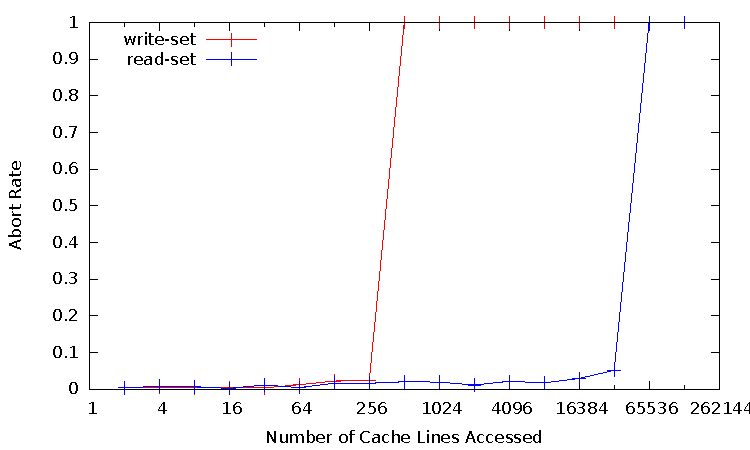
\includegraphics[width=0.75\textwidth,keepaspectratio]{trxSize_singleThread}
    \caption{\textbf{TSX RTM abort rate versus cache lines accessed for a single thread on
        one core}}\label{fig:trx_size} 
\end{figure}

It is clear that transactions abort 100\% of the time once the thread tries to write to
512 or more cache lines within the transaction.  This is consistent with the size of the
L1 cache, 32KB of 64 bytes caches lines equates to 512 cache lines; it is unrealistic to
expect that no other process will use the cache while the transaction is executing and
thus the transaction cannot occupy the cache in its entirety.  Note that the cache is
split into 64 8-way sets; if memory is not organized properly, the total write-set size
will be reduced.

It is evident that the same size limitations do not hold for the read-set size.  While
eviction of a cache line containing a write-set address will always cause a transactional
abort, eviction of a cache line containing a read-set address may not cause an immediate
transactional abort; these cache lines may be tracked by a second-level structure in the
L2 cache \cite{intel_opt_man}.

The objective of the second benchmark is to evaluate the read and write-set sizes for a
transaction being executed by a single thread on a shared core, \emph{i.e., a
  hyper-threaded core}.  This benchmark uses the same procedure as above, but with two
threads bound to the same core.  Each thread accesses the same number of cache lines, but
at different memory locations to prevent any data conflicts. Figure~\ref{fig:trx_size_ht}
shows the abort rate for one of the threads as the number of cache lines accessed within
each transaction increases.

\begin{figure}[H]
    \centering
    \graphicspath{ {./figures/} }
    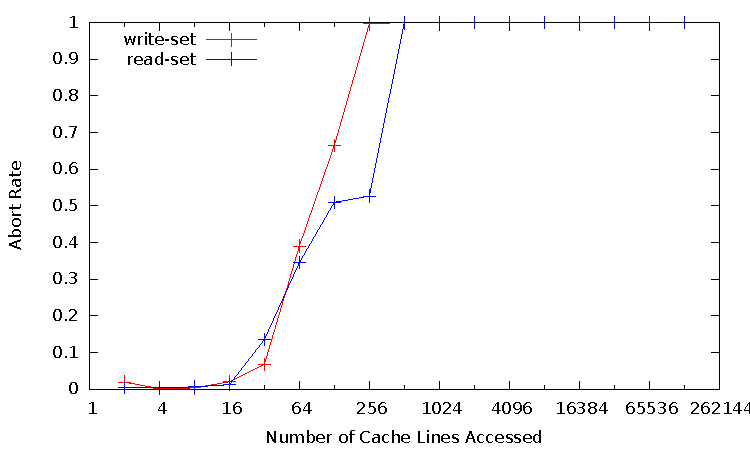
\includegraphics[width=0.75\textwidth,keepaspectratio]{trxSize_hyperthreaded}
    \caption{\textbf{TSX RTM abort rate versus cache line accesses for two threads on
        hyper-threaded core.}}\label{fig:trx_size_ht}
\end{figure}

It is evident that the write-set is strictly limited to half of the L1 cache.  However,
the probability of an abort is non-trivial for any write-set size between 32 and 128 cache
lines.  It is also evident that the read-set size is limited to a similar size as the
write-set on a hyper-threaded core.

\section{Transaction Duration}

Transaction aborts can be caused by a number of run-time events \cite{intel_prog_ref},
including but not limited to: interrupts, page faults, I/O operations, context switches,
illegal instructions, etc.  This is due to the inability of the processor to save the
transactional state information \cite{schwahn}.

The objective of the third benchmark is to evaluate the running time restrictions for a
transaction, \emph{i.e.}, how long can a transaction safely execute without failing.  The
duration of each transaction is increased by increasing the number of operations performed
within the transaction. The critical section performs a certain number of increment
operations on a single data element in the body of loop.  The loop increments to a limit
specified by the duration being tested.  The operation count or duration is increased
logarithmically from 1000 to 1000000 every iteration of the main test loop.
Figure~\ref{fig:trx_duration} shows the transaction abort rate as the duration of the
transaction is increased.

\begin{figure}[H]
    \centering
    \graphicspath{ {./figures/} }
    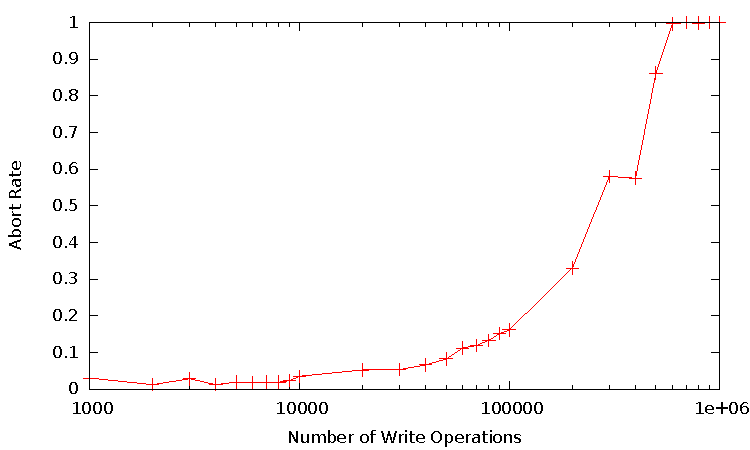
\includegraphics[width=0.75\textwidth,keepaspectratio]{trxDuration}
    \caption{\textbf{TSX RTM abort rate versus number of operations performed during
        transaction.}}\label{fig:trx_duration}
\end{figure}

It is clear that the longer a transaction executes, the higher the probability is that it
will abort.  Practical applications will perform a varying number of operations that take
varying amounts of time.  This benchmark simply demonstrates there is a limit to how long
a transaction can be executed.  Shorter transactions are more likely to succeed than
longer transactions.

\section{Synchronization Latency}

Conventional synchronization mechanisms have varying latencies, therefore TSX most likely
also has varying latencies.  While it is incredibly difficult to obtain accurate
measurements, the objective of this benchmark is to compare the TSX latencies to
conventional synchronization mechanism latencies.  This benchmark merely demonstrates how
long TSX synchronization mechanisms take to enter a transactional region relative to how
long conventional synchronization mechanisms take to enter a critical section.

Each synchronization mechanism is used to perform a simple increment operation.  The
thread calls the locking function, increments the data, and calls the release function
100000 times.  The execution time of the entire loop is measured using the
\texttt{gettimeofday} functionality in Linux.  The locking/release functions use one of
the following depending on the configuration:

\vspace*{-\bigskipamount}
\begin{singlespace}
\begin{enumerate}
  \item no synchronization,
  \item an atomic compare and exchange lock,
  \item a mutex lock,
  \item HLE, and
  \item RTM.
\end{enumerate}
\end{singlespace}

\noindent
The results are shown in Figure~\ref{fig:tsx_latency}.  Clearly the HLE and RTM mechanisms
take longer to actually complete the synchronization process.  This can most likely be
attributed to the extra actions performed by the hardware to initiate transactional
execution.

%need to make image cleaner
\begin{figure}[H]
    \centering
    \graphicspath{ {./figures/} }
    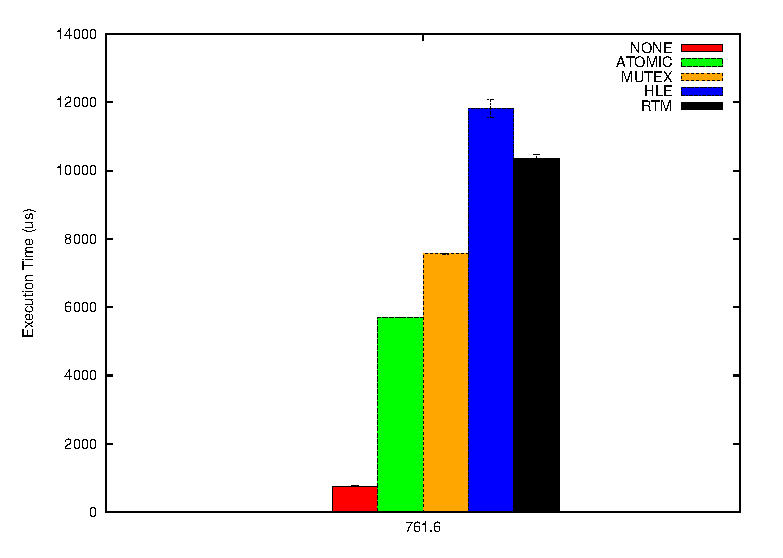
\includegraphics[width=0.75\textwidth,keepaspectratio]{SyncBM}
    \caption{\textbf{Synchronization Latency}}\label{fig:tsx_latency}
\end{figure}

\section{Nesting Transactions}

When developing larger TSX enabled multi-threaded applications, it is possible for
critical sections to be nested within one another.  TSX supports nested transactions for
both HLE and RTM regions, as well as a combination of the two.  When the processor
encounters an \texttt{XACQUIRE} instruction prefix or an \texttt{XBEGIN} instruction, it
increments a nesting count.  Note that the processor transitions to transactional
execution when the nesting count goes from 0 to 1 \cite{intel_prog_ref}.  When the
processor encounters an \texttt{XRELEASE} instruction prefix or an \texttt{XEND}
instruction, the nesting count is decremented.  Once the nesting count returns to 0, the
processor attempts to commit the transactions as one monolithic transaction
\cite{intel_prog_ref}.

The total nesting depth is still limited by the physical resources of the hardware.  If
the nesting count exceeds this implementation specific limit, the transaction may abort.
Upon abort, the processor transitions to non-transactional execution as if the first lock
instruction was executed without elision \cite{intel_prog_ref}.

Scenarios may arise where different locks may be nested within the same critical section.
For instance, one critical section may reside within a separate critical section.  While
this is not a concern for RTM regions, it can become a concern for HLE regions, as the
processor can only track a fixed number of HLE prefixed locks.  However, any HLE prefixed
locks executed after this implementation specific limit has been reached will simply
execute without elision; consequently, the secondary lock variable will be added to the
transaction's write-set \cite{intel_prog_ref}.


\chapter{PDES and \textsc{warped}}

\section{Background}

Discrete Event Simulation (DES) models a system's state changes at discrete points in
time.  In a DES model, physical processes are represented by Logical Processes (LPs)
\cite{des_misra}.  For example, in an epidemic simulation, LPs represent geographical
locations containing a subset of the total population.  The LP's state represents the
diffusion of the disease within the location and the status of the occupants at that
location.  Executed Events in this simulation represent the arrival or departure of
individuals to or from that location, the progression of a disease within an individual at
that location, the diffusion of a disease throughout that location, etc
\cite{epidemic}. To effectively model epidemics, a significant population size and number
of locations needs to be simulated.

In general, DES simulators consist of the following data structures \cite{fujimoto}:

\vspace*{-\bigskipamount}
\begin{singlespace}
\begin{itemize}
  \item\textbf{Pending Event Set}: contains events that have been scheduled, but not
    processed.  Events are retrieved from this structure to be executed.
  \item\textbf{Clock}: denotes how far the simulation has progressed.
  \item\textbf{State}: describes the state of the system.
\end{itemize}
\end{singlespace}

\noindent
The state of the simulation can only change upon execution of an event.  During the
execution of an event, the simulation: 

\vspace*{-\bigskipamount}
\begin{singlespace}
\begin{enumerate}
  \item retrieves the least time-stamped event from the pending event set,
  \item processes the event, 
  \item updates the LP's state, and 
  \item if necessary, inserts generated events into the pending event set.
\end{singlespace}

The need for large simulation models has energized research in Parallel Discrete Event
Simulation (PDES).  Events from separate LPs are executed concurrently by one of \emph{N}
threads.  Each LPs' events execute in chronological order to ensure local causality
constraints are met \cite{fujimoto}.  However, PDES is susceptible to other causality
errors.  Optimistically synchronized simulators are the most susceptible to these
causality errors.  While conservatively synchronized simulators do not execute events
until the system has determined it is safe to do so \cite{fujimoto}, optimistic
approaches, such as the Time Warp protocol, detect rather than prevent causal errors. The
advantage of optimistic approaches is increased concurrency as events are continually
executed until a causal error is detected.

One of the most well-known optimistic protocols is the Time Warp mechanism
\cite{fujimoto}.  In addition to the standard DES data structures, each LP in a simulation
implementing the Time Warp protocol consists of the following data structures:

\vspace*{-\bigskipamount}
\begin{singlespace}
\begin{itemize}
  \item \textbf{Unprocessed Queue}: contains events that have been scheduled, but have yet
    to be executed.  This structure acts as the pending event set for the LP.
  \item\textbf{Processed Queue}: records previously executed events.
  \item\textbf{Output Queue}: contains event messages sent to other LPs.
\end{itemize}
\end{singlespace}

In Time Warp, a causality error occurs if an event message is received containing an event
time-stamp smaller than the time-stamp of the previously executed event.  Such an event is
known as a \emph{straggler} event.  When a straggler event is received by an LP, that LP
must undo all effects of all events executed with a time-stamp greater than that of the
straggler event, henceforth referred to as a \emph{rollback}.  During a rollback,
prematurely executed events are removed from the processed queue and reinserted into the
unprocessed queue after the straggler event.  For every event message in the output queue
with an event time-stamp greater than that of the straggler event, an \emph{anti-message}
is generated.  Anti-messages are sent to the associated LP of that event and remove the
prematurely generated event from the remote LP's queue.
Figure~\ref{fig:rollback_stragglerrecvd} shows the scheduling state of the LP as a
straggler event is received.  Figure~\ref{fig:rollback_processed} shows the scheduling
state of the LP after the rollback is processed \cite{dickman}.

\begin{figure}[H]
    \centering
    \graphicspath{ {./figures/} }
    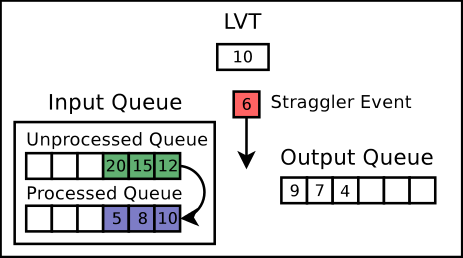
\includegraphics[width=0.5\textwidth,keepaspectratio]{rollback_recv}
    \caption{\textbf{LP at the time of a straggler event is
        received}}\label{fig:rollback_stragglerrecvd}
\end{figure}

\begin{figure}[H]
    \centering
    \graphicspath{ {./figures/} }
    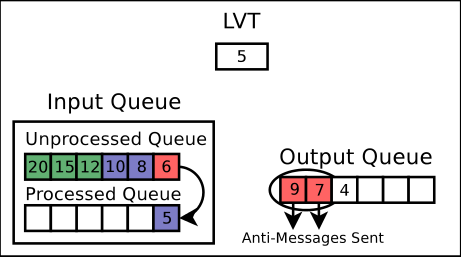
\includegraphics[width=0.5\textwidth,keepaspectratio]{rollback_processed}
    \caption{\textbf{LP after a rollback is processed}}\label{fig:rollback_processed}
\end{figure}

While rollbacks are a problem in themselves, rollbacks represent another issue relevant to
this study; the need to access the pending event set.  When a rollback modifies an LP's
local pending event set, the global pending event set must be updated as well.  Any access
to the global pending event set is a possible point of contention as only one thread can
access this structure at a time.  The implementation and management of the pending event
set is crucial to the overall performance of PDES \cite{twpes}.

\section{The \textsc{warped} Pending Event Set}

\textsc{warped} is a publicly available Discrete Event Simulation (DES) kernel
implementing the Time Warp protocol \cite{martin,fujimoto}.  It was recently redesigned
for parallel execution on multi-core processing nodes \cite{muthalagu}.  It has many
configuration options and utilizes many different algorithms of the Time Warp protocol
\cite{fujimoto}.

%% JOSH: a figure illustrating the pending event set here would facilitate the
%% description. 

The pending event set is maintained as a two-level structure in \textsc{warped}
\cite{dickman}.  Each LP maintains its own event set as a time-stamp ordered
queue.  As previously mentioned, each LP maintains an unprocessed queue for
scheduled events yet to be executed and a processed queue to store previously
executed events.  A common Least Time-Stamped First queue is populated with the
least time stamped event from each LP's unprocessed queue.  As the name
suggests, the LTSF queue is automatically sorted in increasing time-stamp order
so that worker threads can simply retrieve an event from he head of the queue.
This guarantees the worker thread retrieves the least time-stamped event without
having to search through the queue. The LTSF queue is also referred to as the
schedule queue in \textsc{warped}; these terms will be used interchangeably.

%% PHIL stopped here....

\subsection{Pending Event Set Data Structures}

The implementation of the pending event set is a key factor in the performance
of the simulation \cite{twpes}.  The \textsc{warped} simulation kernel has two
functional implementations: 1) the C++ Standard Template Library (STL) multi-set
data structure, and 2) the splay tree data structure.  The way in which these
data structures are accessed and, more importantly, self-adjust will be relevant
to how effectively TSX can be used to access these structures.

\paragraph{STL Multi-set}

The STL multi-set data structure , specifically the sorted STL multi-set data
structure, is an abstract data structure implemented as a self-balancing,
red-black binary search tree \cite{redblack}.  Look-up, insertion, and
deletion operations performed in a red-black tree with \emph{n} elements are
performed in average O(log n) time.  When insertion or deletion operations are
performed, the tree is rebalanced by a tree rearrangement algorithm and a
"painting" algorithm taking average O(1) and O(log n) time respectively. 

The STL multi-set is a self sorting data structure.  The lowest value element
will always be the left most child node of the tree.  To access the least
time-stamped event at the head of the LTSF queue, multi-set red-black tree must
be traversed to the left most child node.  Any insertion or removal of events
requires the red-black tree to rebalance itself.  

\paragraph{Splay Tree}

The splay tree is a self-adjusting binary search tree in which recently accessed
elements are moved to the root of the tree for quicker access \cite{splaytree}.
Look-up, insertion, and deletion operations performed in a splay tee with
\emph{n} elements are performed in average O(log n) time.  When an element is
inserted or looked up, a splaying operation is to move that element to the root
of the tree.

When an event is inserted into the LTSF queue, it becomes the root of the splay
tree.  While this is advantageous if it is known that the root of the tree is
the next least time-stamped event, the tree will have to be most of the time.
If it is known that the next event to be scheduled is the located at the root of
the tree, the worker thread scheduling the event can simply retrieve the node at
the root of the tree without performing any searching operations.  This will
very rarely be the case.  The tree will have to be search when an event is
retrieved to ensure the least time-stamped event is being scheduled.   

\subsection{Worker Thread Event Execution}

A manager thread initiates \emph{n} worker threads at the beginning of the simulation.
It can also suspend inactive worker threads if they run out of useful work.  When a worker
thread is created, or resumes execution after being suspended by the manager thread, it
attempts to lock the LTSF queue and dequeue the least time-stamped event.  If the worker
thread successfully retrieved an event, it executes that event as specified by the
simulation model.  It then attempts to lock the unprocessed queue for the LP associated
with the executed event, and dequeue the next least time-stamped event.  The dequeued
event is inserted into the LTSF queue, which resorts itself based on the event
time-stamps.  An abstract event processing algorithm is shown in Figure
~\ref{workerThreadAlgorithm} \cite{dickman}.  Note that the worker threads perform many
other functions.  The entire pending event set implementation can be seen in Figure
~\ref{fig:singleLTSFqueue} \cite{dickman}.

%Is it legitimate for me to cite figures and pseudocode or do I need to recreate
%these?
\linespread{1.0}
\begin{figure}
\begin{verbatim}
worker_thread()

  lock LTSF queue
  dequeue smallest event from LTSF
  unlock LTSF queue

  while !done loop

    process event (assume from LPi)

    lock LPi queue 

    dequeue smallest event from LPi

    lock LTSF queue

    insert event from LPi
    dequeue smallest event from LTSF

    unlock LTSF queue
    unlock LPi queue
  end loop
\end{verbatim}
\caption{\textbf{Generalized event execution loop for the worker threads.  Many details
    have been omitted for clarity.}}\label{workerThreadAlgorithm}
\end{figure}

\begin{figure}[H]
    \centering
    \graphicspath{ {./figures/} }
    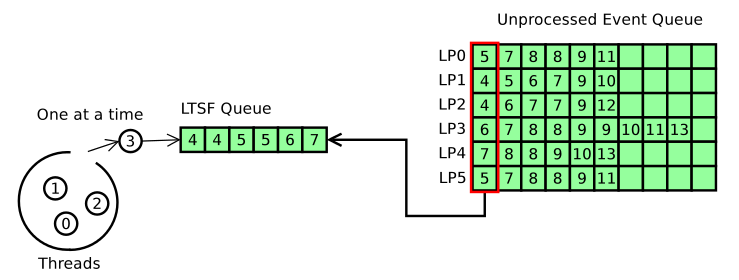
\includegraphics[width=0.75\textwidth,keepaspectratio]{single_ltsf_queue}
    \caption{\textbf{Pending Event Set Scheduling}}\label{fig:singleLTSFqueue}
\end{figure}

\subsection{Contention}

Only one worker thread can access the LTSF queue at a time.  This creates a clear point of
contention during event scheduling as each thread must first retrieve an event from the
LTSF queue.  The LTSF queue must also be updated when events are inserted into any of the
LP pending event sets.  This occurs when new events are generated or the simulation
encounters a causality error and must rollback.

Contention increases with the number of worker threads used to perform the
simulation.  The initial \textsc{warped} implementation execution time was
measured and analyze using 1 to 7 worker threads.  These results can be seen in
Figure ~\ref{fig:notsx_profile}.  It is evident that performance begins to
flatten once the number of worker threads used surpasses four.  This is
attributed to the increased contention for the LTSF queue; with more threads,
each thread has to wait longer for access to the LTSF queue.  The multi-core
processor trend will continue to increase the number of simultaneous execution
threads available, consequently increasing the contention problem.

\begin{figure}[H]
    \centering
    \graphicspath{ {./figures/} }
    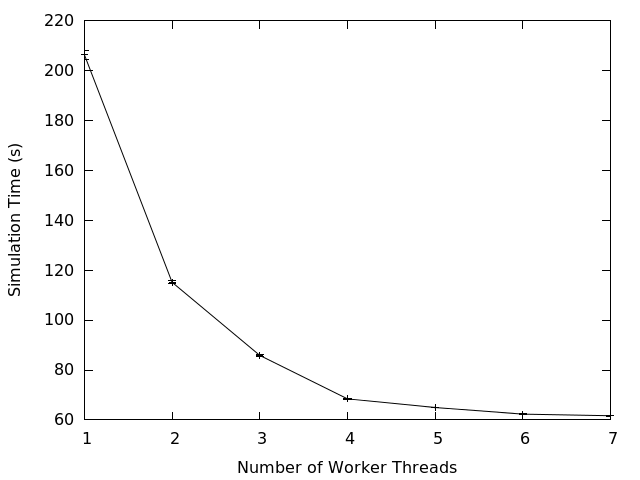
\includegraphics[width=0.75\textwidth,keepaspectratio]{notsx_profile}
    \caption{\textbf{\textsc{warped} Simulation Time versus Worker Thread Count for
        Epidemic Model}}\label{fig:notsx_profile}
\end{figure}

\section{Previous Solutions to Contention}

Dickman \emph{et al} explored the explored the use of various data structures in \textsc{warped}
pending event set implementation, specifically, the STL multi-set, splay tree, and ladder
queue data structures \cite{dickman}.  A secondary focus of this study will expand upon
the use of splay tree versus STL multi-set data structures; at the time of this study, the
ladder queue implementation was being heavily modified and could not be included in this
study.

Another focus of their study was the utilization of multiple LTSF queues \cite{dickman}.
Multiple LTSF queues are created at the beginning of the simulation.  Each LP is assigned
to a specific LTSF queue as shown in Figure~\ref{fig:multipleLTSF}.  In a simulation
configured with four LPs, two worker threads, and two LTSF queues, two LPs and one thread
are assigned to each queue.  This significantly reduced contention as each thread could
access separate LTSF queues concurrently.  The initial implementation statically assigned
LPs to LTSF queues.  This resulted in an unbalanced load distribution, leading to an
increased number of rollbacks and reduced simulation performance.  This was corrected
using a load balancing algorithm to dynamically reassign LPs to LTSF queues.  This study
expands the previous multiple LTSF queue to evaluate if contention can be reduced even
further with TSX.

\begin{figure}[H]
    \centering
    \graphicspath{ {./figures/} }
    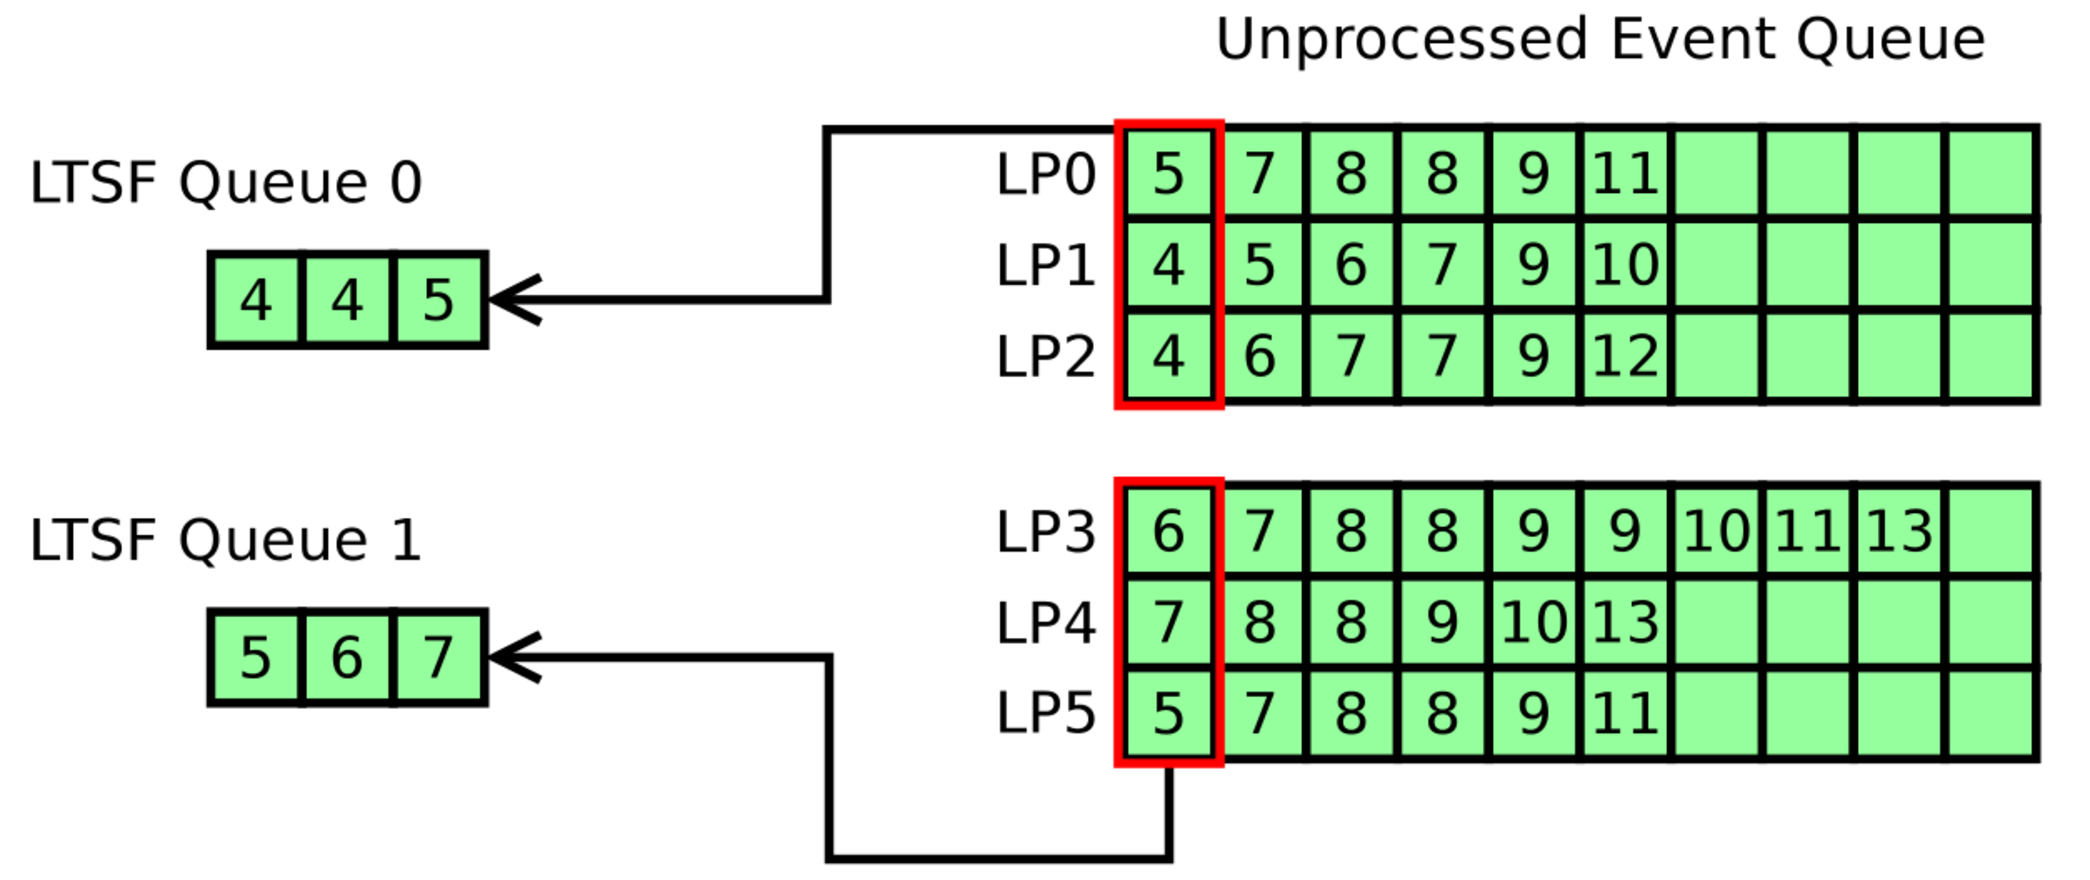
\includegraphics[width=0.75\textwidth,keepaspectratio]{multiple_ltsf}
    \caption{\textbf{Pending Event Set Scheduling with Multiple LTSF
        Queues}}\label{fig:multipleLTSF}
\end{figure}

\section{Thread Migration}

Another potential solution to contention is to distribute worker threads that
try to simultaneously access the same LTSF queue to different LTSF queues.  In
the original scheduling scheme, worker threads are assigned to a specific LTSF
queue.  The worker thread would insert the next event into the same LTSF it had
just scheduled from as seen in Figure ~\ref{workerThreadAlgorithm}.  In this
implementation, the worker thread inserts the next event into a different LTSF
queue, based on a circularly incremented counter.  This approach dynamically
reassigns worker threads LTSF queues by migrating the threads to new LTSF
queues.  It also implicitly balances the load between the all the LTSF queues.
The number of LTSF queues is specified in a configuration file, and has no
restrictions as in the static assignment.

\linespread{1.0}
\begin{figure}
\begin{verbatim}
worker_thread()

  i = fetch-and-add LTSF queue index
  lock LTSF[i]
  dequeue smallest event from LTSF[i]
  unlock LTSF[i]

  while !done loop

    process event (assume from LPi)

    lock LPi queue
    
    dequeue smallest event from LPi

    i = fetch-and-add LTSF queue index

    lock LTSF[i]

    insert event from LPi into LTSF[i]
    dequeue smallest event from LTSF[i]

    unlock LTSF queue
    unlock LPi queue
  end loop
\end{verbatim}
\caption{\textbf{Generalized event execution loop for migrating worker threads.  Many
    details have been omitted for clarity.}}\label{migratinWorkerThreadAlgorithm}
\end{figure}

It was discovered that this implementation resulted in poor performance on NUMA
architectures.  Jingjing Wang et al. noticed similar performance degradation, which they
attributed to poor memory locality due to the movement of LPs to different threads
\cite{numa}.  To offset these performance hits, a migration count was implemented in this
scheme.  Instead continuous migration, threads would be statically assigned to one LTSF
after executing a certain number of events.

\chapter{\textsc{warped} with TSX}

This section analyzes the various critical sections that use the TSX mechanism.
As previously mentioned, the primary focus of this study is the shared LTSF
queue.  The per LP unprocessed and processed queues also use the TSX mechanism.

\section{\textsc{warped} Critical Sections}

First, it is important to understand the operations performed in a critical
section.  If a critical section always writes to the entire shared data
structure, TSX will most likely not be useful.  Functions are only explained in
terms of the operations pertaining to the specific data structure they operate
on for the sake of clarity.  

\subsection{LTSF Queue Functions}

The following functions require synchronization to access the LTSF
queue:

\begin{itemize}
  \item\texttt{insert()} - insert an event into the LTSF queue if an event was inserted at
    the beginning of a specific LP's unprocessed queue.
  \item\texttt{updatedScheduleQueueAfterExecute()} - inserts the dequeued event from a
    specific LP's unprocessed queue into the LTSF queue.
  \item\texttt{nextEventToBeScheduledTime()} - returns the time of the event at the
    beginning of the LTSF queue.
  \item\texttt{clearScheduleQueue()} - clears the LTSF queue.
  \item\texttt{setLowestObjectPosition()} - \textbf{not clear on this function}
  \item\texttt{peek()} - retrieves the next event for execution.
\end{itemize}

\subsection{Unprocessed Queue Functions}

The following functions require synchronization to access a specific LPs
unprocessed queue:

\begin{itemize}
  \item\texttt{insert()} - insert an event into a specific LP's unprocessed queue.
  \item\texttt{updatedScheduleQueueAfterExecute()} - dequeue the next least time-stamped
    event from a specific LP's unprocessed queue.
  \item\texttt{getEvent()} - dequeue and return the least time-stamped event in the
    unprocessed queue; insert event into processed queue.
  \item\texttt{getEventIfStraggler()} - same as \texttt{getEvent()} but does not insert
    the event into the processed queue as the getEvent function above does.
%need to verify
  \item\texttt{peekEvent()} - return a reference to the next event in the LP's unprocessed
    queue.
  \item\texttt{peekEventCoastForward()} - same as \texttt{peekEvent()}.
  \item\texttt{handleAntiMessage()} - delete an event in a specific LP's unprocessed queue
    for which the LP received an anti-message.
  \item\texttt{ofcPurge()} - removes all events from the unprocessed queue; used for
    optimistic fossil collection, which is beyond the scope of this study.
  \item\texttt{peekEventLockUnprocessed()} - peek the first event of a specif LP's
    unprocessed queue, but leave the queue locked.
  \item\texttt{getMinEventTime()} - get the time-stamp of the first event in a specific
    LP's unprocessed queue.
\end{itemize}

\subsection{Processed Queue Functions}

The following functions require synchronization to access a specific LPs
processed queue:

\begin{itemize}
  \item\texttt{getEvent()} - insert the dequeued event from a specific LP's unprocessed
    queue into that LP's processed queue.
  \item\texttt{getEventWhileRollback()} - same as getEvent(), except the unprocessed queue
    is already locked.%need to verify
  \item\texttt{rollback()} - traverse a specific LP's entire processed queue and remove
    any events with a time-stamp greater than or equal to the rollback time; the removed
    events are placed in the LP's unprocessed queue.
  \item\texttt{fossilCollect()} - remove events satisfying a certain criteria from a
    specific LP's processed queue.
  \item\texttt{ofcPurge()} - same as the ofcPurge() function for the unprocessed queue.
\end{itemize}

\section{\textsc{warped} Transactional Regions}

The functions described above perform a variety of memory operations, and any thread can
execute any critical section at any time.  Based on static analysis, there's no way of
knowing which threads will access what structure in what way, hence the need for
synchronization.  But with TSX, functions that do not interfere can execute concurrently.
TSX tracks read and write memory operations separately in the transaction's read-set and
write-set respectively.  Transactions only interfere if a data conflict occurs, \emph{i.e.,} a
thread attempts to write to a memory location in another transaction's read-set, or a
thread attempts to read a memory location in another transaction's write-set.

For example, one worker thread calls \texttt{nextEventToBeScheduleTime} to get the
time-stamp of the event at the head of the LTSF queue.  There is a possibility that a
different worker thread is currently updating the LTSF queue or will attempt to update the
LTSF queue with the first worker thread is in the middle of executing
\texttt{nextEventToBeScheduleTime}.  This scenario necessitates synchronization.  However,
instead of the second worker thread writing to the LTSF queue, it also calls
\texttt{nextEventToBeScheduleTime}.  Both are read operations and do not interfere with
each other.  TSX recognizes this scenario and allows the worker threads to execute
concurrently, whereas locks force one worker thread to wait until the other is done with
the LTSF queue.

Several similar scenarios can arise during simulation execution. While there are too many
possible scenarios to identify specifically where TSX can be beneficial, the potential to
expose concurrency through dynamic synchronization is too great to be dismissed. Note,
there is also no guarantee that TSX will work 100\% of the time; there are several
run-time events that can cause transactions to abort, as well as physical limitations.

% The next 3-4 paragraphs might be bull shit, I'm not really sure yet.  I
% wrote this at 5am and just started spewing out thoughts relating TSX to my
% limited understanding of the multiset and splay tree data structures.
% I also haven't decided if the results are significant enough to even talk
% about the different schedule queue implementations.
The process of scheduling requires a significant amount of write operations to
the queues listed above.  As long as executing threads do not write to an entire
queue, there is a good chance that the write operations will not interfere.  TSX
dynamically determines if the write operations are performed on different memory
locations and allows the threads to execute concurrently.  The data structures
used to implement the respective queues is a significant factor in determining
if two or more threads perform conflicting memory operations on the same
structure.  Not only is the performance of simulation dependent on the pending
event set implementation, but the performance of TSX is also dependent on the
data structures implementing the pending event set.

For example, a worker thread is scheduling the next least time-stamped event
from the LTSF queue and needs to remove that event from the queue.  In the STL
multi-set schedule queue implementation, the tree must be traversed to the
lowest value element, which adds all tree nodes in that path to the transactions
read-set.  The node is removed, but the STL multi-set must go through the
process of rebalancing itself before the transaction ends.  Before the multi-set
can complete the rebalancing process, another worker thread attempts to schedule
the next least time-stamped event. It traverse the tree to the lowest value
element and removs it.  This involves a write operation to the parent node of
the event.  But the node was already addded to the first transaction's read-set.
A data conflict results and both transactions must abort.

In the splay tree schedule queue implementation, the next least time-stamped event
is already the root of the splay tree, either because it was just peeked at or
inserted.  A worker thread enters the transaction to schedule the event and
remove it from the queue.  The splay tree must be traversed to ensure that the
least time-stamped event is being scheduled, thus adding the entire structure to
the read-set of the transaction.  This increases the likelihood of a data
conflict should any other thread try to write to the tree in any way while the
original transaction is executing.

Both of these data structures are some form of binary tree.  It is possible for
very few nodes to be accessed during certain operations, especially the
multi-set red-black tree.  This is advantageous for TSX as less memory locations
will not be added to the transaction read-sets thus making it less likely for
data conflicts to occur.   

It is possible, though highly unlikely, that either implementation could take
the form of a single linked list, depending on what order events are inserted
in.  For instance, events inserted into the multi-set red-black tree in
increasing chronological order create a singly linked list. This situation poses
a threat to TSX if the entire list is traversed in a transaction.  Not only
because access to any element becomes a possible data conflict, but also because
of size limitations.  If the LTSF queue contains too many events, TSX might not
be able to track all the memory locations involved in the queue, thus resulting
in aborts.

\section{TSX Implementation}

This section discusses how both TSX interfaces were implemented in \textsc{warped}.

\subsection{Hardware Lock Elision (HLE)}

The generic algorithm presented in Figure~\ref{fig:hle_interface} in Section~\ref{sec:hle}
only works for locks with a binary value, \emph{i.e.,} the lock is free or not free.  The
\textsc{warped} locking mechanism assigns the thread number to the lock value to indicate
which thread currently holds the lock.  To comply with this implementation, custom HLE
lock acquire and lock release functions were implemented.  GCC inline assembly functions
were developed appending the appropriate HLE prefixes to a lock cmpxchg instruction.

\subsection{Restricted Transactional Memory (RTM)}

As previously explained in Section~\ref{sec:rtm}, RTM allows the programmer to
specify an abort path to be executed upon a transactional abort.  This allows
better tuning of RTM performance.  The RTM algorithm implemented in
\textsc{warped} includes a retry algorithm described below in Figure
~\ref{rtm_retry}. Instead of immediately retrying transactional execution, the
algorithm decides when and if the transaction should be retried based on the
condition of the abort.  If the transaction was explicitly aborted for reasons
other than another thread owning the lock, do not retry transactional execution.
The programmer used the \texttt{\_xabort()} function to explicitly abort the
transaction. If the lock was not free upon entering the transaction, wait until
it is free to retry transactional execution.  If a data conflict occurred, wait
an arbitrary amount of time before retrying.  This offsets the execution of the
conflicting threads in hopes that the conflicting memory operations will be
performed at different times on the next retry.

The RTM retry limit is specified at compile time.  Each data structure maintains its own
retry limit initially set to the global limit.  A backoff algorithm is used to reduce the
retry limit for a specific data structure.  If the transactions for this data structure
abort more often than not, the retry limit is reduced.  If the transaction
commit rate increases, the retry limit increases up to the inital limit
specified at compile time.  This ideally reduces the number of transaction
attempts for an extended period of time.  The retry limit increases if the
commit rate passes the abort to commit rate ratio threshold

Furthermore, if transactions for the data structure consistently abort for an extended
period of time with no successfull commits, transactional execution is not attempted for
the remainder of the simulation.

\begin{figure}
\begin{verbatim}
while retry count is less than retry limit
    status = _xbegin()

    if status == XBEGIN
        if lock is free
            execute transactional region
        else
            _xabort

    update abort stats

    if transaction will not succeed on retry or 
        _xabort was called due to reasons other than the lock not being free

        break

    else if _xabort was used because the lock was not free

        wait until the lock becomes free to retry

    else if a data conflict occurred
        
        wait an arbitrary amount of time before retrying

    increment retry count
end loop

acquire lock

execute critical section
\end{verbatim}
\caption{\textbf{RTM Retry Algorithm}}\label{rtm_retry}
\end{figure}

\chapter{Experimental Analysis}

This study compares the performance of the \textsc{warped} simulation kernel
using conventional synchronization mechanisms, Hardware Lock Elision, and
Restricted Transactional memory.  All simulations were performed on a system
with an Intel i7-4770 running at 3.4 GHz with 32GB of RAM.  Average execution
time and standard deviation were calculated from a set of 10 trials for each
simulation configuration.

The simulation model used to obtain the following results is an epidemic model.  It
consists of 110998 geographically distributed people in 119 separate locations requiring a
total of 119 LPs.  The epidemic is modeled by reaction processes to model progression of
the disease within an individual entity, and diffusion processes to model transmission of
the disease among individual entities.

\section{The Default Multi-set Schedule Queue}

The default implementation of the LTSF queue is the STL multi-set data
structure.  It is a self-adjusting binary search tree which keeps the least
time-stamped event in the left most leaf node of the tree.

\subsection{Static Thread Assignment}

In the original \textsc{warped} thread scheduling scheme, threads are
statically assigned to an LTSF queue.  Contention will clearly be a problem if
the simulation only schedules from one LTSF queue as every worker thread is
assigned to that queue.

The first part of this study compares the performance of the \textsc{warped}
pending event set static thread scheduling implementation using one LTSF queue
synchronized with : 1) atomic locks, 2) HLE, and 3) RTM with 1 retry, 4) RTM
with 9 retries, and 5) RTM with 19 retries.  These results are shown in Figure
~\ref{fig:noThrMig_timeVSthreads_1schq}.  It is clear that using HLE improves
simulation performance, but still suffers from the same rise in contention as
the number of worker threads is increased.
%TODO: discuss RTM results

\begin{figure}[H]
    \centering
    \graphicspath{ {./figures/} }
    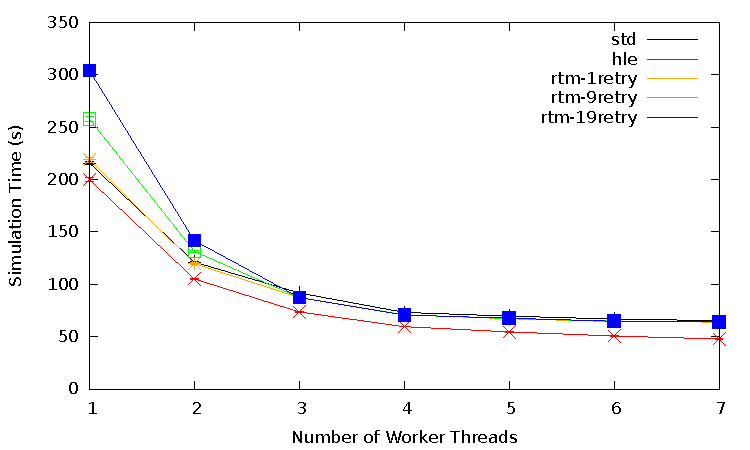
\includegraphics[width=0.75\textwidth,keepaspectratio]{hugeepidemicsim-NOmig-timeVSthreads-multiset-1schQ}
    \caption{\textbf{Simulation Time versus Number of Worker Threads 1 STL Multi-set LTSF Queue}}
    \label{fig:noThrMig_timeVSthreads_1schq}
\end{figure}

It is evident from Figure ~\ref{fig:noThrMig_timeVSthreads_1schq} that
contention is increasing as the number of worker threads increases, regardless
of the synchronization mechanism used.  This is somewhat expected as contention
is still high for the single LTSF queue.  Transactional memory exposes
concurrency where it can, but some critical sections simply cannot be executed
concurrently.  It should be noted that the performance of HLE does not flatten
quite as much as the other synchronization mechanisms.

The initial solution to alleviate contention for the LTSF queue is the
utilization of multiple LTSF queues.  The data for different numbers of schedule
queues is limited by the necessity to have a number of LTSF queues evenly
divisble by the number of worker threads.  This is because of the way threads
are assigned to LTSF queues; if the numbers are not evenly divisible, the
simulation becomes unbalanced.  LPs assigned to a certain LTSF queue can get far
ahead or behind of other LPs on LTSF queue resulting in significant rollbacks
and thus performance degradation.  The various LTSF queue count configuration
results are shown in Tables ~\ref{tab:noThrMig_2threadsXschq},
~\ref{tab:noThrMig_3threadsXschq}, ~\ref{tab:noThrMig_5threadsXschq}, and Figures
~\ref{fig:noThrMig_timeVSschq_4threads} and
~\ref{fig:noThrMig_timeVSschq_6threads}.

The only configuration that seems to alleviate contention is two LTSF queues
with 2 or 6 worker threads.  The other configurations result in increased
simulation times.  The rollback counts for these configurations were also
consideraly high.  These poor performance could be attributed to the lack of a
proper load balancing procedure.\par

\begin{table}[H]
    \centering
    \begin{tabular}{l|p{2cm}|p{2cm}|p{2cm}|p{2cm}|p{2cm}}
        \textbf{\# LTSF Queues}&Lock &HLE &RTM-1retry &RTM-9retry &RTM-19retry \\
        \hline
        \midrule
            1 &121.2255  &105.0569 &119.6892 &131.3282 &141.6453 \\ 
            2 &118.1558  &101.1242 &114.1276 &128.93   &144.2886 \\
    \end{tabular}
    \caption{\textbf{Simulation Times for 2 Worker Threads with X LTSF Queues}}
    \label{tab:noThrMig_2threadsXschq}
\end{table}

\begin{table}[H]
    \centering
    \begin{tabular}{l|p{2cm}|p{2cm}|p{2cm}|p{2cm}|p{2cm}}
        \textbf{\# LTSF Queues}&Lock &HLE &RTM-1retry &RTM-9retry &RTM-19retry \\
        \hline
        \midrule
            1 &91.68472 &73.58687 &87.36819 &87.34794 &87.38973 \\ 
            3 &89.50474 &70.24289 &84.21861 &94.00537 &104.4246 \\
    \end{tabular}
    \caption{\textbf{Simulation Times for 3 Worker Threads with X LTSF Queues}}
    \label{tab:noThrMig_3threadsXschq}
\end{table}

\begin{figure}[H]
    \centering
    \graphicspath{ {./figures/} }
    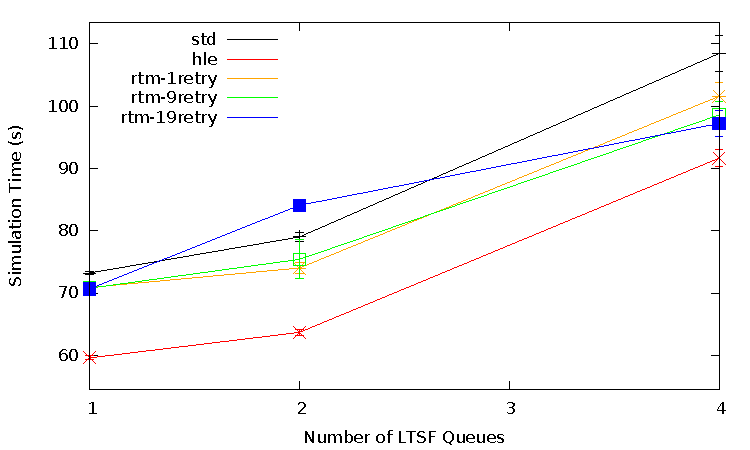
\includegraphics[width=0.75\textwidth,keepaspectratio]{hugeepidemicsim-NOmig-timeVSschedQs-multiset-4thread}
    \caption{\textbf{Simulation Time versus Number of STL Multi-set LTSF Queues for 4
        Worker Threads}}\label{fig:noThrMig_timeVSschq_4threads}
\end{figure}

\begin{table}[H]
    \centering
    \begin{tabular}{l|p{2cm}|p{2cm}|p{2cm}|p{2cm}|p{2cm}}
        \textbf{\# LTSF Queues}&Lock &HLE &RTM-1retry &RTM-9retry &RTM-19retry \\
        \hline
        \midrule
            1 &69.62144  &54.59489 &67.10837 &67.34648 &67.61373\\ 
            5 &93.21429  &76.85048 &89.62641 &76.4832  &72.18505\\
    \end{tabular}
    \caption{\textbf{Simulation Times for 5 Worker Threads with X LTSF
        Queues}}\label{tab:noThrMig_5threadsXschq}
\end{table}

\begin{figure}[H]
    \centering
    \graphicspath{ {./figures/} }
    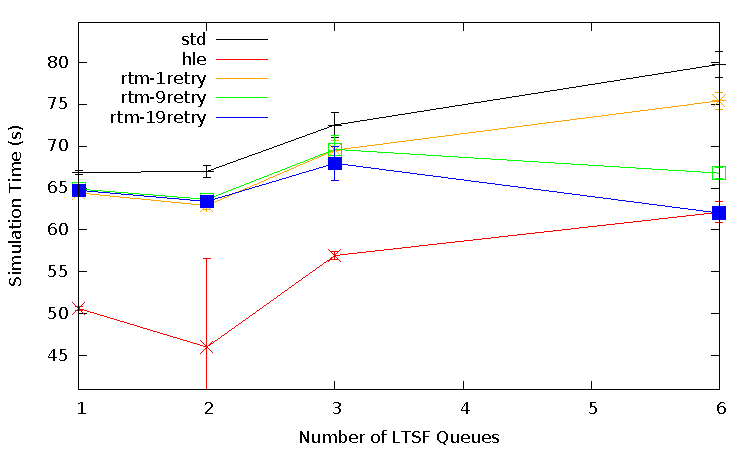
\includegraphics[width=0.75\textwidth,keepaspectratio]{hugeepidemicsim-NOmig-timeVSschedQs-multiset-6thread}
    \caption{\textbf{Simulation Time versus Number of STL Multi-set LTSF Queues for 6
        Worker Threads}}\label{fig:noThrMig_timeVSschq_6threads}
\end{figure}

\subsection{Dynamic Thread Assignment}

Another solution to contention is to distribute worker threads that try to
simultaneously access the same LTSF queue to different LTSF queues.  Worker
threads are dynmically assigned to LTSF queues rather than statically.  

\subsubsection{Continuous Thread Migration}

The first solution continuously reassigns worker threads to the next  
This solution implicitly balances the work load between LTSF queues.  Therefore,
any number of LTSF queues can be used with any number of worker threads.  These
results are shown in Table ~\ref{tab:contThrMig_2threadsXschq} and Figures
~\ref{fig:contThrMig_timeVSschq_3threads} through
~\ref{fig:contThrMig_timeVSschq_7threads}. 

It is evident that this scheduling scheme slightly improves performance
increasing the number of LTSF queues from 1 to 4.  Increasing the number of LTSF
queues beyond 4 does not seem to significantly improve performance.  The
performance of HLE synchronization, while still superior ,seems to follow the
same trend as standard synchronization mechanisms.
%TODO: more discussion maybe?

\begin{table}[H]
    \centering
    \begin{tabular}{l|p{2cm}|p{2cm}|p{2cm}|p{2cm}|p{2cm}}
        \textbf{\# LTSF Queues}&Lock &HLE &RTM-1retry &RTM-9retry &RTM-19retry \\
        \hline
        \midrule
            1 &121.4532  &105.2221 &118.95   &131.0166 &139.4046 \\ 
            2 &122.5693  &105.7831 &118.8288 &130.422  &141.834  \\
    \end{tabular}
    \caption{\textbf{Simulation Times for 2 Worker Threads with X LTSF
        Queues}}\label{tab:contThrMig_2threadsXschq}
\end{table}

\begin{figure}[H]
    \centering
    \graphicspath{ {./figures/} }
    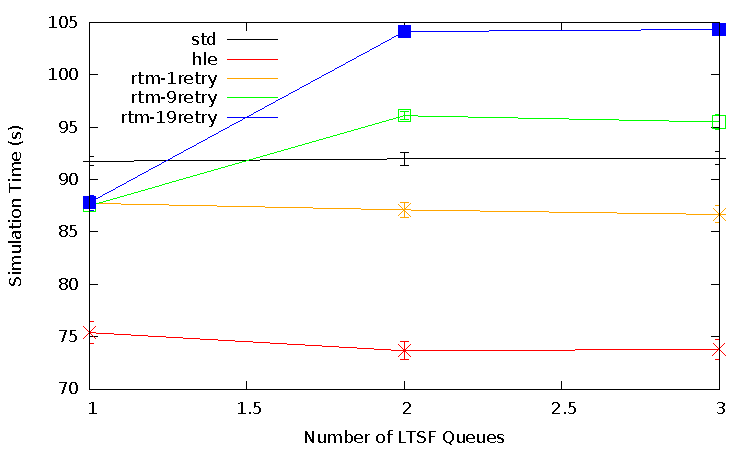
\includegraphics[width=0.75\textwidth,keepaspectratio]{hugeepidemicsim-CONTmig-timeVSschedQs-multiset-3thread}
    \caption{\textbf{Simulation Time versus Number of STL Multi-set LTSF Queues for 3
        Worker Threads}}\label{fig:contThrMig_timeVSschq_3threads}
\end{figure}

\begin{figure}[H]
    \centering
    \graphicspath{ {./figures/} }
    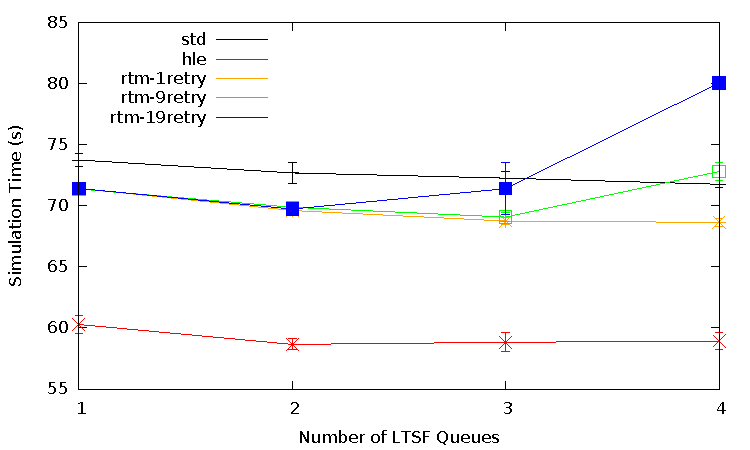
\includegraphics[width=0.75\textwidth,keepaspectratio]{hugeepidemicsim-CONTmig-timeVSschedQs-multiset-4thread}
    \caption{\textbf{Simulation Time versus Number of STL Multi-set LTSF Queues for 4
        Worker Threads}}\label{fig:contThrMig_timeVSschq_4threads}
\end{figure}

\begin{figure}[H]
    \centering
    \graphicspath{ {./figures/} }
    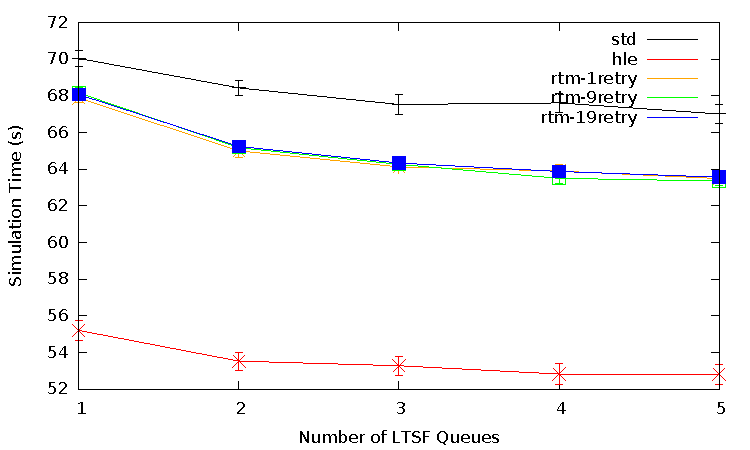
\includegraphics[width=0.75\textwidth,keepaspectratio]{hugeepidemicsim-CONTmig-timeVSschedQs-multiset-5thread}
    \caption{\textbf{Simulation Time versus Number of STL Multi-set LTSF Queues for 5
        Worker Threads}}\label{fig:contThrMig_timeVSschq_5threads}
\end{figure}

\begin{figure}[H]
    \centering
    \graphicspath{ {./figures/} }
    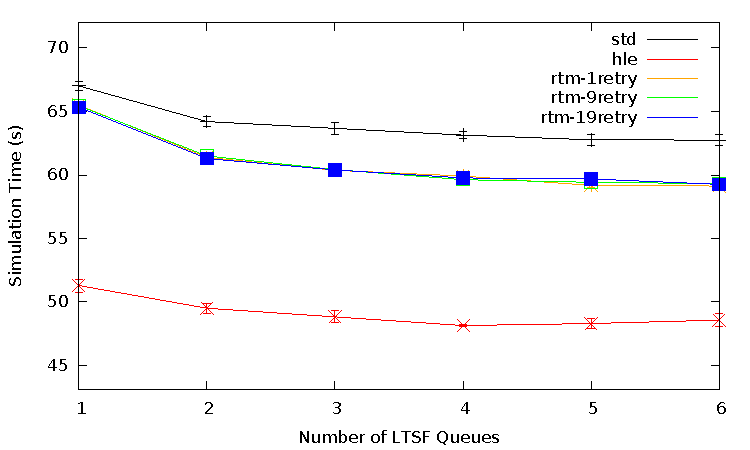
\includegraphics[width=0.75\textwidth,keepaspectratio]{hugeepidemicsim-CONTmig-timeVSschedQs-multiset-6thread}
    \caption{\textbf{Simulation Time versus Number of STL Multi-set LTSF Queues for 6
        Worker Threads}}\label{fig:contThrMig_timeVSschq_6threads}
\end{figure}

\begin{figure}[H]
    \centering
    \graphicspath{ {./figures/} }
    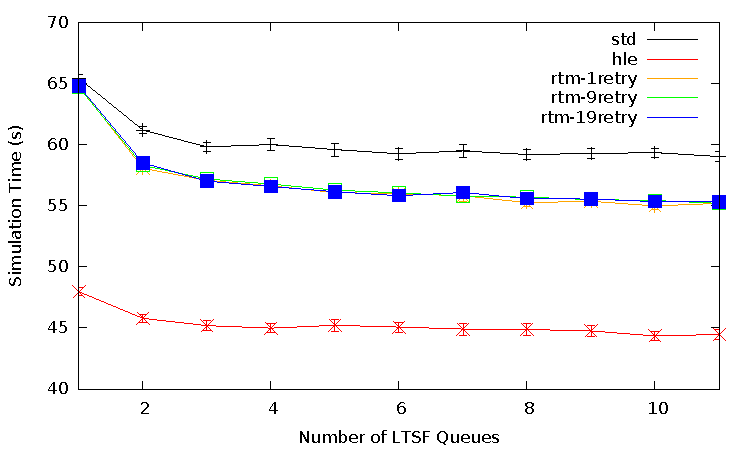
\includegraphics[width=0.75\textwidth,keepaspectratio]{hugeepidemicsim-CONTmig-timeVSschedQs-multiset-7thread}
    \caption{\textbf{Simulation Time versus Number of STL Multi-set LTSF Queues for 7
        Worker Threads}}\label{fig:contThrMig_timeVSschq_7threads}
\end{figure}

\subsubsection{Event Limited Thread Migration}

As previously discussed, the continuous thread migration approach does not work
well for NUMA architectures due to memory locality issues.  The thread migration
scheme was modified to migrate threads between LTSF queues for the first 50
events a thread executes.  The threads continue to schedule from the same LTSF
queue they executed the fiftieth event from.  

While the continous migration scheme is not problematic for the system under
test, the comparison was made to thoroughly evaluate TSX using this scheme as a
viable solution to contention.  TSX may also one day become available on NUMA
architectures.  Further testing would need to be performed, but at least it will
be known if this solution has any significant impact on contention.  These
results are shown in Tables ~\ref{tab:xThrMig_2threadsXschq},
~\ref{tab:xThrMig_3threadsXschq}.  ~\ref{tab:xThrMig_5threadsXschq}, and Figures
~\ref{fig:xThrMig_timeVSschq_4threads} and
~\ref{fig:xThrMig_timeVSschq_6threads}.

It is evident that any static thread to LTSF queue assignment suffers from the
same problems.  Except for the 2 worker thread, 2 LTSF queue and 3 worker
thread, 3 LTSF queue configurations, performance suffers as the number of LTSF
queues is increased.  This is most likely attributed more to lack of adequate
load balancing than contention.

\begin{table}[H]
    \centering
    \begin{tabular}{l|p{2cm}|p{2cm}|p{2cm}|p{2cm}|p{2cm}}
        \textbf{\# LTSF Queues}&Lock &HLE &RTM-1retry &RTM-9retry &RTM-19retry \\
        \hline
        \midrule
            1 &121.2448  &105.6107 &124.1983 &123.6149 &123.0078\\ 
            2 &117.6654  &102.0753 &121.0667 &137.9824 &154.3929\\
    \end{tabular}
    \caption{\textbf{Simulation Times for 2 Worker Threads with X LTSF
        Queues}}\label{tab:xThrMig_2threadsXschq} 
\end{table}

\begin{table}[H]
    \centering
    \begin{tabular}{l|p{2cm}|p{2cm}|p{2cm}|p{2cm}|p{2cm}}
        \textbf{\# LTSF Queues}&Lock &HLE &RTM-1retry &RTM-9retry &RTM-19retry \\
        \hline
        \midrule
            1 &92.36592  &74.22306 &93.23531  &92.67724 &92.6402 \\ 
            3 &88.91337  &70.67712 &89.53974  &107.369  &126.557 \\
    \end{tabular}
    \caption{\textbf{Simulation Times for 3 Worker Threads with X LTSF
        Queues}}\label{tab:xThrMig_3threadsXschq} 
\end{table}

\begin{figure}[H]
    \centering
    \graphicspath{ {./figures/} }
    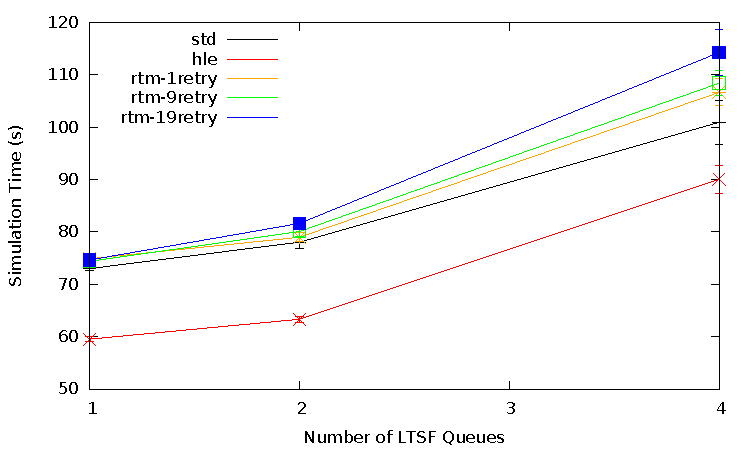
\includegraphics[width=0.75\textwidth,keepaspectratio]{hugeepidemicsim-XEVENTmig-timeVSschedQs-multiset-4thread}
    \caption{\textbf{Simulation Time versus Number of STL Multi-set LTSF Queues for 4
        Worker Threads}}\label{fig:xThrMig_timeVSschq_4threads}
\end{figure}

\begin{table}[H]
    \centering
    \begin{tabular}{l|p{2cm}|p{2cm}|p{2cm}|p{2cm}|p{2cm}}
        \textbf{\# LTSF Queues}&Lock &HLE &RTM-1retry &RTM-9retry &RTM-19retry \\
        \hline
        \midrule
            1 &69.30301  &54.40232 &70.85832  &70.46488 &70.4784 \\ 
            5 &95.31338  &77.55966 &93.71796  &85.63724 &76.2384 \\
    \end{tabular}
    \caption{\textbf{Simulation Times for 5 Worker Threads with X LTSF
        Queues}}\label{tab:xThrMig_5threadsXschq}
\end{table}

\begin{figure}[H]
    \centering
    \graphicspath{ {./figures/} }
    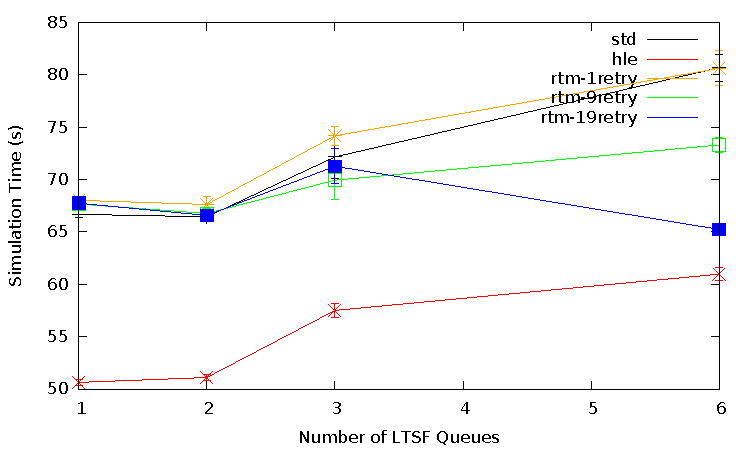
\includegraphics[width=0.75\textwidth,keepaspectratio]{hugeepidemicsim-XEVENTmig-timeVSschedQs-multiset-6thread}
    \caption{\textbf{Simulation Time versus Number of STL Multi-set LTSF Queues for 6
        Worker Threads}}\label{fig:xThrMig_timeVSschq_6threads}
\end{figure}

\subsubsection{Migration Scheme Comparison}

Figures~\ref{fig:migComp_4threads} through \ref{fig:migComp_7threads} show the comparison
of the migration schemes used.

\begin{figure}[H]
    \centering
    \graphicspath{ {./figures/} }
    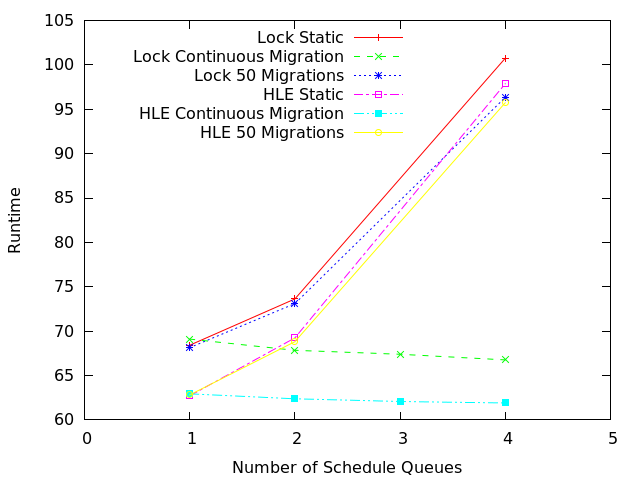
\includegraphics[width=0.75\textwidth,keepaspectratio]{migComp_4threads}
    \caption{\textbf{Comparison of Migration Schemes for 4 Worker Threads with X LTSF
        Queues}}\label{fig:migComp_4threads}
\end{figure}

\begin{figure}[H]
    \centering
    \graphicspath{ {./figures/} }
    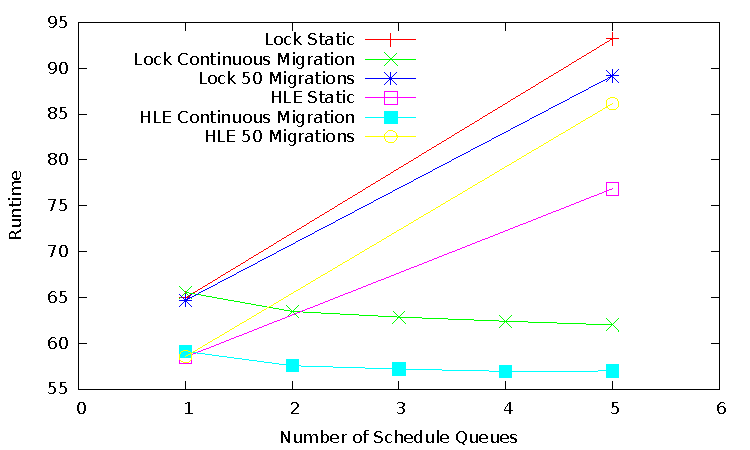
\includegraphics[width=0.75\textwidth,keepaspectratio]{migComp_5threads}
    \caption{\textbf{Comparison of Migration Schemes for 5 Worker Threads with X LTSF
        Queues}}\label{fig:migComp_5threads}
\end{figure}

\begin{figure}[H]
    \centering
    \graphicspath{ {./figures/} }
    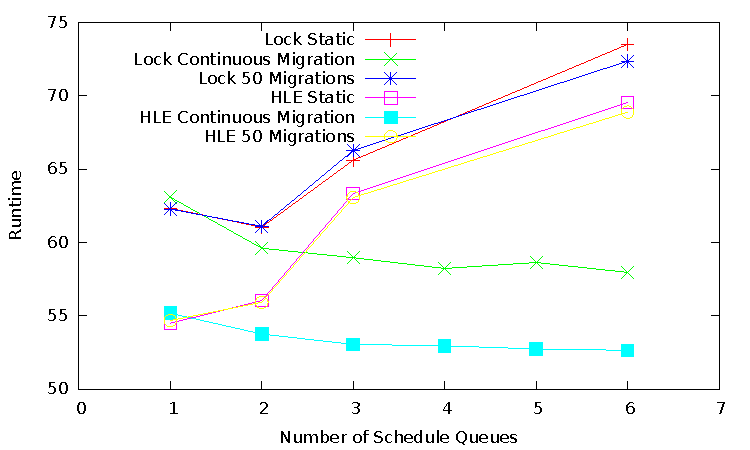
\includegraphics[width=0.75\textwidth,keepaspectratio]{migComp_6threads}
    \caption{\textbf{Comparison of Migration Schemes for 6 Worker Threads with X LTSF
        Queues}}\label{fig:migComp_6threads}
\end{figure}

\begin{figure}[H]
    \centering
    \graphicspath{ {./figures/} }
    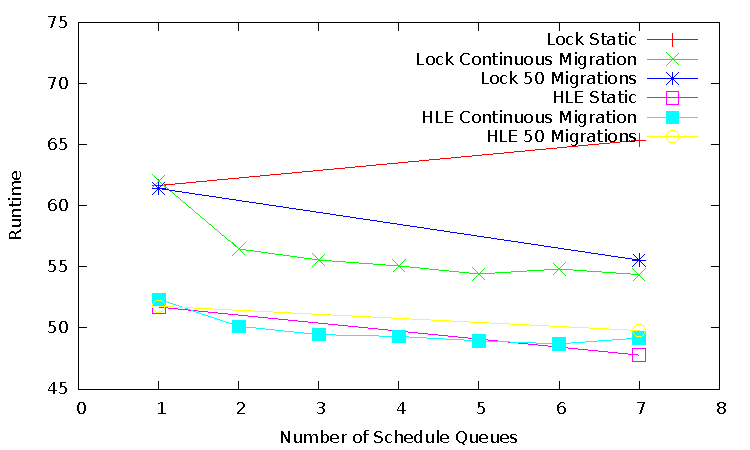
\includegraphics[width=0.75\textwidth,keepaspectratio]{migComp_7threads}
    \caption{\textbf{Comparison of Migration Schemes for 7 Worker Threads with X LTSF
        Queues}}\label{fig:migComp_7threads}
\end{figure}

\section{The Splay Tree Implementation}

The data structure used to implement the pending event set is a factor in the performance
of the overall simulation.  First, the difference between the two data structures is
demonstrated for standard synchronization methods.  These results are shown in Tables
~\ref{tab:noThrMig_2threadsXschq_msVSst_std}, \ref{tab:noThrMig_3threadsXschq_msVSst_std},
\ref{tab:noThrMig_5threadsXschq_msVSst_std}, and
Figures~\ref{fig:noThrMig_timeVSschq_4threads_msVSst_std} and
\ref{fig:noThrMig_timeVSschq_6threads_msVSst_std}.

It is evident that the splay tree implementation performs better for one LTSF
queue, but becomes comparable to the multi-set performance as the number of LTSF
queues is increased.  
%TODO: why

\begin{table}[H]
    \centering
    \begin{tabular}{l|p{2cm}|p{2cm}|p{2cm}|p{2cm}}
        \textbf{\# LTSF Queues}&Multi-Set &Std Err &Splay Tree &Std Err\\
        \hline
        \midrule
            1 &121.2255  &0.709044 &115.8633  &0.560395\\ 
            2 &118.1558  &0.870117 &115.6354  &0.614937\\
    \end{tabular}
    \caption{\textbf{Multi-Set VS Splay Tree LTSF Queues for Standard Synchronization
        Mechanisms using 2 Worker Threads}}\label{tab:noThrMig_2threadsXschq_msVSst_std}
\end{table}

\begin{table}[H]
\centering
\begin{tabular}{l|p{2cm}|p{2cm}|p{2cm}|p{2cm}}
    \textbf{\# LTSF Queues}&Multi-Set &Std Err &Splay Tree &Std Err\\
    \hline
    \midrule
        1 &91.68472  &0.623036 &86.40983  &0.361082\\ 
        3 &89.50474  &0.390017 &86.52189  & 0.969298\\
\end{tabular}
\caption{\textbf{Multi-Set VS Splay Tree LTSF Queues for Standard Synchronization
    Mechanisms using 3 Worker Threads}}\label{tab:noThrMig_3threadsXschq_msVSst_std}
\end{table}

\begin{figure}[H]
    \centering
    \graphicspath{ {./figures/} }
    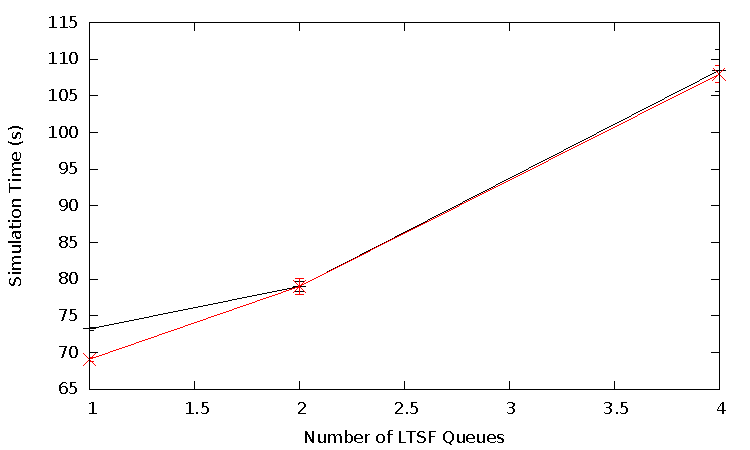
\includegraphics[width=0.75\textwidth,keepaspectratio]{hugeepidemicsim-NOmig-timeVSschedQs-msVSst-4thread-std}
\caption{\textbf{Multi-Set VS Splay Tree LTSF Queues for Standard Synchronization
    Mechanisms using 4 Worker Threads}}\label{fig:noThrMig_timeVSschq_4threads_msVSst_std}
\end{figure}

\begin{table}[H]
\centering
\begin{tabular}{l|p{2cm}|p{2cm}|p{2cm}|p{2cm}}
    \textbf{\# LTSF Queues}&Multi-Set &Std Err &Splay Tree &Std Err\\
    \hline
    \midrule
        1 &69.62144   &0.283633 &65.40437   &0.180788\\ 
        5 &93.21429   &1.972659 &95.41614   &1.331701\\
\end{tabular}
\caption{\textbf{Multi-Set VS Splay Tree LTSF Queues for Standard Synchronization
    Mechanisms using 5 Worker Threads}}\label{tab:noThrMig_5threadsXschq_msVSst_std}
\end{table}

\begin{figure}[H]
    \centering
    \graphicspath{ {./figures/} }
    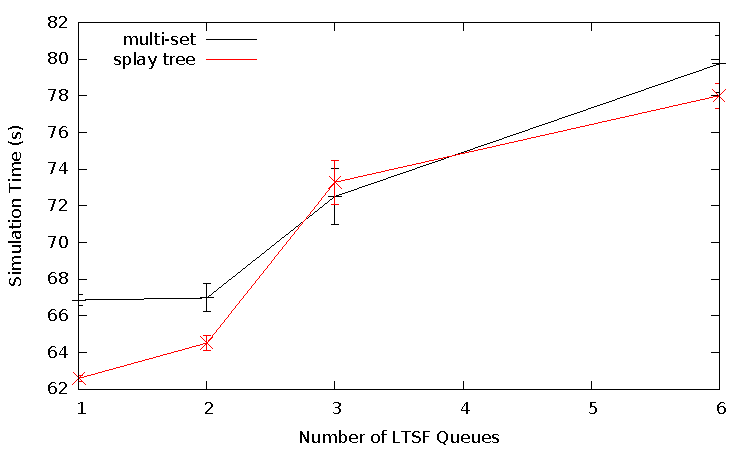
\includegraphics[width=0.75\textwidth,keepaspectratio]{hugeepidemicsim-NOmig-timeVSschedQs-msVSst-6thread-std}
\caption{\textbf{Multi-Set VS Splay Tree LTSF Queues for Standard Synchronization
    Mechanisms using 6 Worker Threads}}\label{fig:noThrMig_timeVSschq_6threads_msVSst_std}
\end{figure}

The data structure used to implement the LTSF queue will also impact how TSX performs.
These results are shown in Tables~\ref{tab:noThrMig_2threadsXschq_msVSst_hle},
\ref{tab:noThrMig_3threadsXschq_msVSst_hle}.  \ref{tab:noThrMig_5threadsXschq_msVSst_hle},
and Figures~\ref{fig:noThrMig_timeVSschq_4threads_msVSst_hle} and
\ref{fig:noThrMig_timeVSschq_6threads_msVSst_hle}.

For a single LTSF queue, the splay tree implementation performs slightly better
than the multi-set implementation.  However, the splay tree performs
noticeably worse than the multi-set when more than one LTSF queue is used
with HLE synchronization.  

\begin{table}[H]
    \centering
    \begin{tabular}{l|p{2cm}|p{2cm}|p{2cm}|p{2cm}}
        \textbf{\# LTSF Queues}&Multi-Set &Std Err &Splay Tree &Std Err\\
        \hline
        \midrule
            1 &105.0569   &0.866889 &102.51192  &1.22734  \\ 
            2 &101.12417  &0.616301 &93.12871   &21.783966\\
    \end{tabular}
    \caption{\textbf{Multi-Set VS Splay Tree LTSF Queues for HLE TSX using 2 Worker
        Threads}}\label{tab:noThrMig_2threadsXschq_msVSst_hle}
\end{table}

\begin{table}[H]
\centering
\begin{tabular}{l|p{2cm}|p{2cm}|p{2cm}|p{2cm}}
    \textbf{\# LTSF Queues}&Multi-Set &Std Err &Splay Tree &Std Err\\
    \hline
    \midrule
        1 &73.58687   &0.45751  &72.57065   &0.449519\\ 
        3 &70.24289   &0.665394 &70.4064    &0.729255\\
\end{tabular}
\caption{\textbf{Multi-Set VS Splay Tree LTSF Queues for HLE TSX using 3 Worker
    Threads}}\label{tab:noThrMig_3threadsXschq_msVSst_hle}
\end{table}

\begin{figure}[H]
    \centering
    \graphicspath{ {./figures/} }
    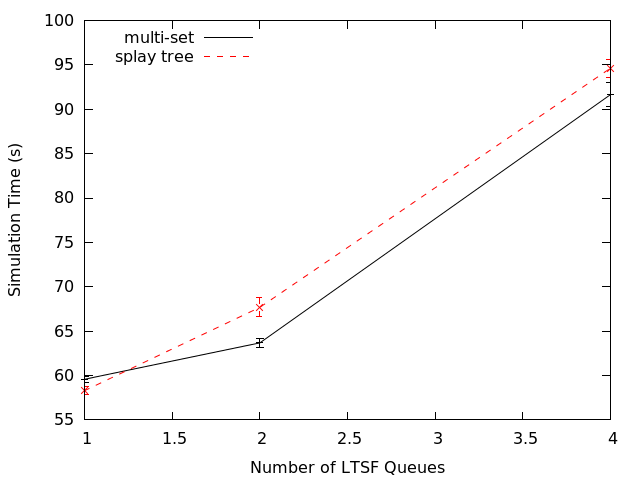
\includegraphics[width=0.75\textwidth,keepaspectratio]{hugeepidemicsim-NOmig-timeVSschedQs-msVSst-4thread-hle}
\caption{\textbf{Multi-Set VS Splay Tree LTSF Queues for HLE TSX using 4 Worker
    Threads}}\label{fig:noThrMig_timeVSschq_4threads_msVSst_hle}
\end{figure}

\begin{table}[H]
\centering
\begin{tabular}{l|p{2cm}|p{2cm}|p{2cm}|p{2cm}}
    \textbf{\# LTSF Queues}&Multi-Set &Std Err &Splay Tree &Std Err\\
    \hline
    \midrule
        1 &54.59489   &0.331819 &53.25156   &0.280322\\ 
        5 &76.85048   &1.975723 &81.47112   &1.135243\\
\end{tabular}
\caption{\textbf{Multi-Set VS Splay Tree LTSF Queues for HLE TSX using 5 Worker
    Threads}}\label{tab:noThrMig_5threadsXschq_msVSst_hle}
\end{table}

\begin{figure}[H]
    \centering
    \graphicspath{ {./figures/} }
    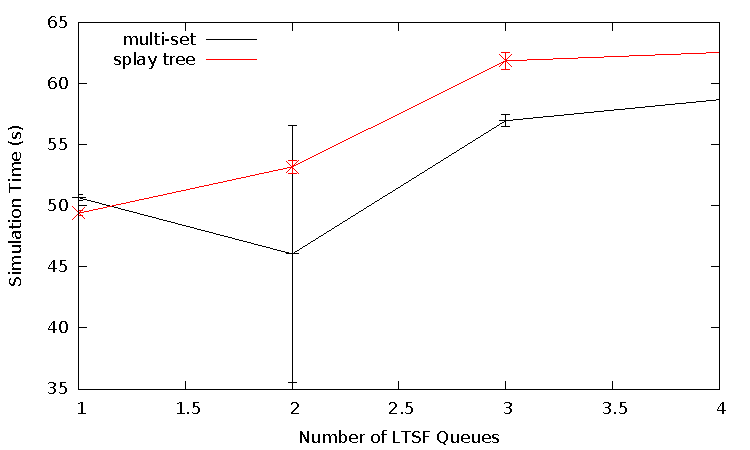
\includegraphics[width=0.75\textwidth,keepaspectratio]{hugeepidemicsim-NOmig-timeVSschedQs-msVSst-6thread-hle}
\caption{\textbf{Multi-Set VS Splay Tree LTSF Queues for HLE TSX using 6 Worker
    Threads}}\label{fig:noThrMig_timeVSschq_6threads_msVSst_hle}
\end{figure}

%TODO: compare RTM 

\chapter{Discussion}

This thesis explored the use of Intel's transactional memory implementation,
Transactional Synchronization Extensions (TSX) in the multi-threaded
\textsc{warped} PDES kernel to alleviate contention for the pending event set.
The \textsc{warped} pending event set consists of a global Least Time-Stamped
First (LTSF) queue and local event set queues for each LP.  The LTSF queue, the
processed queues, and unprocessed queues were modified to use standard and TSX
synchronization mechanisms. 

\section{Conclusions}

Based on the results above, it clear that TSX improved performance of
\textsc{warped}.  HLE consistently shows speedup over conventional
synchronization mechanisms.  It even slightly reduces execution time when the
simulation only uses one LTSF queue.  In other configurations, HLE reduces
execution time by as much as 20\%. 

RTM performance trends were much less consistent.  The number of RTM retries was
varied to better tune the performance of RTM.  In some configurations, the
simulation time as the number of retries inceased also increase, while in other
configurations the simulation time decreased as the number of retries increased.
There were also configurations where the simulation did not change significantly
as the number of retries was increased.  Regardless, RTM still showed speedup
over conventional synchronization mechanisms in most configurations, even though
it was not nearly as much speedup as HLE.  The inconsistencies in speedup trends
as well as overall speedup can most likely be attributed to the overhead
associated with RTM.  The retry algorithm requires abort statistics to be
calculated and maintained which adds a bit more overhead to RTM.  Furthermore,
the backup algorithm modifies the number of retries allowed, thus varying the
actual number of retries attempted between simulations with even the same
configuration.

Increasing the number of LTSF queues from 1 to 2 usually resulted in reduced
contention and thus improved performance.  Increasing the LTSF queue to anything
greater than 2 usually resulted in performance degradation in the migration
schemes involving static thread assignment.  This is due to the
lack of adequate load balancing procedures.  The continuous migration scheme did
show performance improvements increasing the LTSF queue up to 4, but leveled
off with any number of LTSF queues greater than 4.  

The multi-set data structure performed better than splay tree data structure
when using TSX synchronization mechanisms.  The splay tree usually has to
traverse the whole tree for the least time-stamped event, or at least to ensure
the least time-stamped event is being scheduled.  This adds a majority of the
data in the tree to the read-set of transactions, thus increasing the chances of
data conflicts and memory overflows with respect to the transactional memory
tracking.

In conclusion, TSX significantly improves simulation performance for the
\textsc{warped} PDES kernel.  While other solutions to contention also improved
performance, they did not seem to have a significant impact on how TSX
performed.  The speedup introduced by TSX was fairily consistent between the
three migration schemes.

\section{Future Work}

\subsection{LTSF Queue Implementation}

The LTSF queue was only implemented with two different data structures in this
study.  The ladder queue implementation was still being developed at the time of
this writing.  The ladder queue performs faster insertions and deletions, as
well as provides new opportunities for alternative synchronization methods. 
%I don't know much about this, need some help here.

\subsection{Transactionally Designed Critical Sections}

\textsc{warped} was not designed with transactional memory in mind.  The
critical sections described above were designed based on the notion that they
would be protected by locks and executed sequentially by the threads.
Transactional memory changes that mindset.  Programming with concurrency in mind
could allow transactional memory to perform more effectively.

\subsection{More Models}

At the time of this study, only the epidemic simulation model was working well
enough to be tested.  Several other models have been developed for
\textsc{warped}, such as a RAID model and several circuit simulation models, but
are going through rigorous development.  Future studies should explore other
models as the very nature of the model could impact the performance of TSX in
any configuration described above.

\newpage
\bibliographystyle{abbrv}
\bibliography{refs}

\end{document}
